\documentclass[10pt]{article}
% Language setting
% Replace `english' with e.g. `spanish' to change the document language
\usepackage[spanish]{babel}

% Set page size and margins
% Replace `letterpaper' with`a4paper' for UK/EU standard size
\usepackage[a4paper,top=1.9cm,bottom=3.67cm,left=1.9cm,right=1.32cm,marginparwidth=1.75cm]{geometry}

% Useful packages
\usepackage{amsmath}
\usepackage{graphicx}
\usepackage[colorlinks=true, allcolors=blue]{hyperref}

% Set document Font
\usepackage{fontspec}

\setmainfont{Times New Roman}

% Para las ecuaciones: https://latex.codecogs.com/eqneditor/editor.php?lang=es-es

\title{Proyecto Global Integrador AyME:\\
Control de Accionamiento de CA con Motor Sincrónico de Imanes Permanentes}

\author{Guarise Renzo, Trubiano Lucas\\
Profesor: Ing. Gabriel L. Julián\\
\\
Universidad Nacional de Cuyo - Facultad de Ingeniería\\
Automática y Máquinas Eléctricas\\
Ingeniería Mecatrónica}

\begin{document}
\maketitle

\begin{center} % Centrar texto
    {\Large \textbf{Resumen}}
\end{center}

En el presente proyecto se modelará, diseñará, analizará y simulará un sistema de control automático de posición y movimientos para un accionamiento electromecánico de 4 cuadrantes compuesto por una máquina eléctrica de corriente alterna (CA) trifásica sincrónica con excitación por imanes permanentes (PMSM), la cual es alimentada por un inversor trifásico desde una fuente ideal de corriente continua (CC) y un reductor de velocidad de engranajes planetarios de salida hacia la carga mecánica. Se dispone además un sensor de posición (encoder) en el eje del motor, 3 sensores de corriente instantánea de fases en la salida del inversor al estator y un sensor de temperatura del bobinado de estator. La carga mecánica es el brazo de un robot tipo SCARA, para el cual no se ha considerado la dinámica NL a modo de simplificación. Como primera instancia se modelará el sistema completo. Luego se hará un profundo análisis de este, estudiando sus no linealidades, acoplamientos y su comportamiento ante la incertidumbres en sus parámetros. Por último, se llevará a cabo una estrategia de control vectorial con campo orientado a partir de la cual se diseñará un controlador externo de movimiento en cascada con un modulador de torque.


% \tableofcontents % Creamos el indice

\section{Introducción}


\section{Desarrollo}
\subsection{Modelado, Análisis y Simulación dinámica del SISTEMA FÍSICO a “Lazo Abierto” (Sin Controlador externo de Movimiento)}
\subsubsection{Modelo matemático equivalente (1 GDL) del subsistema mecánico completo}
En el sistema físico real hay varios subsistemas mecánicos los cuales detallaremos a continuación para luego hacer una combinación de todos estos en un único subsistema mecánico equivalente.

\begin{itemize}
	\item \textbf{Carga mecánica}\vspace{0.3cm}\\
	En lo que refiere al subsistema mecánico del brazo del robot y la carga mecánica aplicada al mismo, se puede modelar mediante la siguiente ecuación:
	\begin{equation}
		\label{eqn:cargaMecanica}
		J_{l}\cdot \dot{\omega }_{l}\left ( t \right )=T_{q}\left ( t \right )-b_{l}\cdot \omega_{l}\left ( t \right )-T_{l}\left ( t \right )
	\end{equation}
	\begin{equation}
		\omega_{l}\left ( t \right )\equiv \dot{q}_{l}\left ( t \right )= \dot{q}_1\left ( t \right )
	\end{equation}
	Donde $q_{1}(t)$ es la posición articular del hombro del robot, $J_{l}$ es el momento de inercia de todos los eslabones del robot referidos al hombro, $b_{l}$ es el coeficiente de amortiguamiento viscoso, $T_{l}$ es el torque de carga o perturbación y $T_{q}$ es el torque motor entregado a la salida de la caja reductora de engranajes.
	La inercia y el amortiguamiento son dos de los parámetros que varían según la posición de las articulaciones del robot, es decir, $J_{l}(q_{1}(t),q_{2}(t),...,q_{n}(t))$ y una función similar para $b_{l}$.
	En este caso, se considera un valor nominal para estos parámetros, y sus posibles variaciones máximas, pero sin estar relacionado directamente con las posiciones articulares del robot.
	
	\item \textbf{Tren de transmisión:}\vspace{0.3cm}\\
	El tren de transmisión del robot está formado por una caja reductora, reversible, de engranajes planetarios. Se asume acoplamiento \textbf{rígido}, sin elasticidad torsional y sin backlash (juego). Al considerar una transmisión ideal y sin pérdida de potencia, las ecuaciones que la modelan son:
	\begin{equation}
		\label{eqn:relacionTransmision}
		\omega_{l}\left ( t \right )=\frac{1}{r}\cdot w_{m}\left ( t \right )
	\end{equation}
	\begin{equation}
		\label{eqn:torqueTransmision}
		T_{q}\left ( t \right )=r\cdot T_{d}\left ( t \right )
	\end{equation}
	Donde $\omega_{m}(t)$ es la velocidad angular del eje del rotor del motor, $T_{d}(t)$ es el torque de la máquina eléctrica (equivalente a una carga colocada en el eje del rotor) y $r$ es la relación de transmisión del reductor planetario.
	
	\item \textbf{Subsistema mecánico del motor:}\vspace{0.3cm}\\
	Por último tenemos el subsistema mecánico que modela el torque de salida de la máquina eléctrica. Las ecuaciones que modelan el sistema son las siguientes:
	\begin{equation}
		\label{eqn:sistMecanicoMotor}
		J_{m}\cdot \dot{\omega }_{m}\left ( t \right )=T_{m}\left ( t \right )-b_{m}\cdot \omega_{m}\left ( t \right )-T_{d}\left ( t \right )
	\end{equation}
	\begin{equation}
		\omega_{m}\left ( t \right )\equiv \dot{q}_{m}\left ( t \right )
	\end{equation}
	Donde $J_{m}$ es la inercia del rotor respecto a su propio eje, $b_{m}$ es la viscosidad del rotor y $T_{m}(t)$ es el torque electromecánico de la máquina eléctrica.

	\item \textbf{Modelo equivalente mecánico (1 GDL):}\vspace{0.3cm}\\
	A continuación vamos a hacer unas simplificaciones sobre las ecuaciones de los subsistemas mecánicos, con el fin de reducir la complejidad del problema y teniendo en cuenta como hipótesis, que la transmisión es totalmente rígida y sin backlash (juego).
    Esto significa, que todo el movimiento a la entrada del reductor, se transmite a la salida con una relación lineal. Con el torque, sucede lo mismo, hay una transmisión lineal y sin pérdidas de potencia.

	Bajo estas hipotesis, despejamos $T_{d}$ de la ecuación \ref{eqn:torqueTransmision} y lo reemplazamos en la ecuación \ref{eqn:sistMecanicoMotor}:
	\begin{equation}
		\label{eqn:paso1sistMecanico}
		J_{m}\cdot \dot{\omega }_{m}\left ( t \right )=T_{m}\left ( t \right )-b_{m}\cdot \omega_{m}\left ( t \right )-\frac{T_{q}\left ( t \right )}{r}
	\end{equation}
	Luego, despejamos $T_{q}$ de la ecuación \ref{eqn:cargaMecanica} y lo reemplazamos en \ref{eqn:paso1sistMecanico}:
	\begin{equation}
		\label{eqn:paso2sistMecanico}
		J_{m}\cdot \dot{\omega }_{m}\left ( t \right )=T_{m}\left ( t \right )-b_{m}\cdot \omega_{m}\left ( t \right )-\frac{\left ( J_{l}\cdot \dot{\omega_{l}}+b_{l}\cdot \omega_{l}+T_{l} \right )}{r}
	\end{equation}
	Teniendo en cuenta la relación de la ecuación \ref{eqn:relacionTransmision}, la reemplazamos en \ref{eqn:paso2sistMecanico} y reacomodamos la expresión:
	\begin{equation}
		\label{eqn:paso3sistMecanico}
		\left ( J_{m}+\frac{J_{l}}{r^{2}} \right )\cdot \dot{\omega }_{m}\left ( t \right )=T_{m}\left ( t \right )-\left ( b_{m}+\frac{b_{l}}{r^{2}} \right )\cdot \omega_{m}\left ( t \right )-\frac{T_{l}}{r}
	\end{equation}
	Donde establecemos las siguientes equivalencias:
	\begin{equation}
		\label{eqn:Jeq}
		J_{m}+\frac{J_{l}}{r^{2}}=J_{eq}
	\end{equation}
	\begin{equation}
		\label{eqn:beq}
		b_{m}+\frac{b_{l}}{r^{2}}=b_{eq}
	\end{equation}
	\begin{equation}
		\label{eqn:Teq}
		\frac{T_{l}}{r}=T_{eq}
	\end{equation}
	Reemplazando \ref{eqn:Jeq}, \ref{eqn:beq} y \ref{eqn:Teq} en la ecuación \ref{eqn:paso3sistMecanico}, la expresión nos queda:
	\begin{equation}
		\label{sist:mecanico}
		J_{eq}\cdot \dot{\omega }_{m}\left ( t \right )=T_{m}\left ( t \right )-b_{eq}\cdot \omega_{m}\left ( t \right )-T_{eq}
	\end{equation}
	\begin{equation}
		\label{globalNL:omegaM}
		\omega_{m} \equiv \dot{\theta_{m}}
	\end{equation}
	Dicha ecuación se puede representar en bloques de \textbf{Simulink}, como se ve en la siguiente figura \ref{fig:MecanicoEquivalente}:
	\begin{figure}[h!]
		\centering
		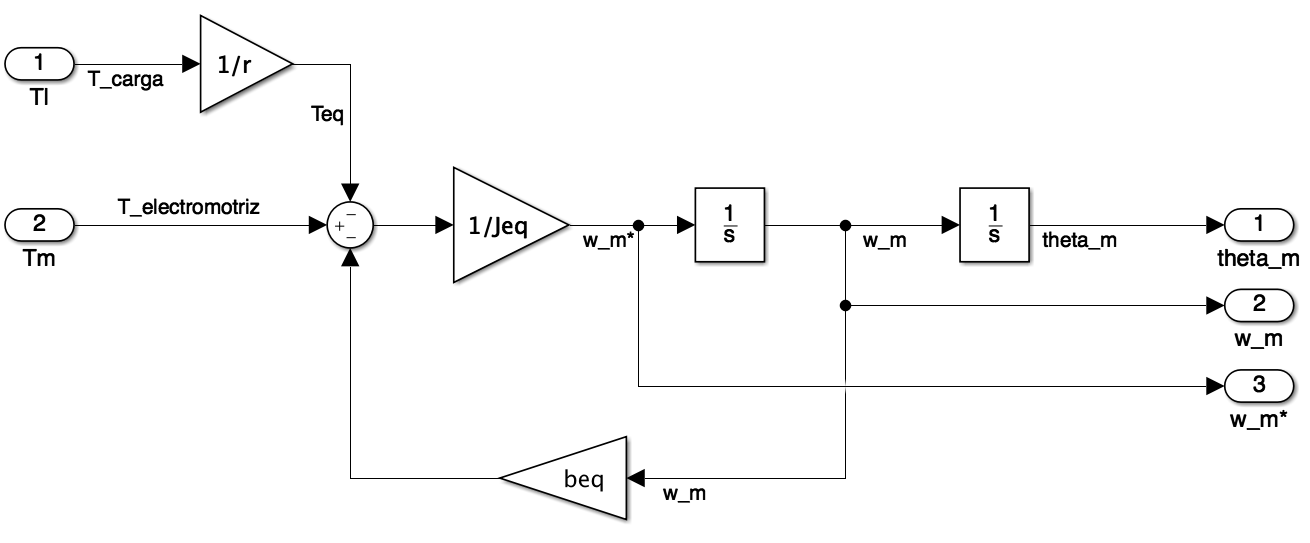
\includegraphics[width=0.5\textwidth]{2_1_1_ModeloMecanicoEquivalente.png}
		\caption{\label{fig:MecanicoEquivalente} Diagrama en bloques del modelo mecánico equivalente simplificado en \textbf{Simulink}}
	\end{figure}

\end{itemize}

\subsubsection{Modelo dinámico del sistema físico completo}

\begin{enumerate}
    \renewcommand{\theenumi}{\alph{enumi}} %Letras minúsculas
    \item \textbf{Modelo global no lineal (NL)}
    
    Para definir el modelo completo del sistema, ya abordamos la parte mecánica. Ahora veamos el resto de los subsistemas para terminar de definir el modelo completo de nuestro sistema físico.
	\begin{itemize}
		\item \textbf{Subsistema Electromagnético:}\vspace{0.3cm}\\
		El motor sincrónico trifásico de CA con excitación por imanes permanentes (PMSM) tiene el estator conectado en estrella (con bornes de fases abcs) y neutro flotante en el centro de la estrella.
		El subsistema es un sistema simétrico al considerar las tres tensiones de fases de igual amplitud y desfasadas 120 grados eléctricos, y equilibrado al poseer de un neutro flotante.
		\vspace{0.3cm}\\
		Para modelar esta máquina, haremos uso de la \textbf{transformación de Park}\footnote[1]{\textbf{Transformación de Park:} forma invariante en módulo de resultante vectorial de variables base $f$} del circuito del estator, llegando así a un modelo idealizado equivalente en coordenadas eléctricas \textbf{qd0} fijas al rotor.
		La transformación de Park nos permite referenciar nuestras variables a un marco de referencia que gira junto al campo eléctrico rotante.
		Y como se trata de un sistema simétrico, luego del transitorio queda totalmente equilibrado, entonces podemos suponer que luego de ese pequeño transitorio $v_{0s}(t)$ tendrá como valor $0$ y se reduce significativamente el número de variables.
		\vspace{0.3cm}\\
		Las coordenadas eléctricas del entrehierro $qd0$, fijas al rotor (marco de referencia “sincrónico”) se definen como:
		\begin{equation}
			\dot{\theta_{r}}\left ( t \right )\equiv \omega_{r}\left ( t \right )\Leftrightarrow \theta_{r}\left ( t \right )=\int_{0}^{t}\omega_{r}\left ( \xi \right )\cdot d\xi + \theta_{r}\left ( 0 \right )
		\end{equation}
		\begin{equation}
			\theta_{r} \left ( t \right ) \equiv P_{p} \cdot \theta_{m} \left ( t \right )
		\end{equation}
		\begin{equation}
			\omega_{r}\left ( t \right )=P_{p}\cdot \omega_{m}\left ( t \right )
		\end{equation}
		El torque electromagnético viene dado por la ecuación:
		\begin{equation}
			\label{sist:electromagnetico}
			T_{m}\left ( t \right )=\frac{3}{2} \cdot P_{p} \cdot \left [ \lambda_{m}^{r'}+\left ( L_{d}-L_{q} \right )\cdot i_{ds}^{r} \left ( t \right ) \right ] \cdot i_{qs}^{r}\left ( t \right )
		\end{equation}
		Donde $\lambda_{m}^{r'}$ es el flujo magnético equivalente de imanes concatenado, por espiras del bobinado de estator,
		$L_{d}$ es la inductancia de eje directo del estator y $L_{q}$ es la inductancia de eje en cuadratura del estator (estas magnitudes son consideradas constantes para simplificar el modelo).
		El modelo equivalente del subsistema eléctrico en coordenadas de entrehierro, está dado por las siguientes ecuaciones, que hacen un balance de tensiones en el circuito del estator.
		\begin{equation}
			\label{sist:electrico1}
			v_{qs}^{r}\left ( t \right )=R_{s}\left ( t \right )\cdot i_{qs}^{r}\left ( t \right )+L_{q}\cdot \frac{\mathrm{d} i_{qs}^{r}\left ( t \right )}{\mathrm{d} t}+\left [ \lambda_{m}^{r'}+L_{d}\cdot i_{ds}^{r}\left ( t \right ) \right ]\cdot \omega_{r}\left ( t \right )
		\end{equation}
		\begin{equation}
			\label{sist:electrico2}
			v_{ds}^{r}\left ( t \right )=R_{s}\left ( t \right )\cdot i_{ds}^{r}\left ( t \right )+L_{d}\cdot \frac{\mathrm{d} i_{ds}^{r}\left ( t \right )}{\mathrm{d} t}-L_{q}\cdot i_{qs}^{r}\left ( t \right )\cdot \omega_{r}\left ( t \right )
		\end{equation}
		\begin{equation}
			\label{eqn:expresionNula}
			v_{0s}^{r}\left ( t \right )=R_{s}\left ( t \right )\cdot i_{0s}^{r}\left ( t \right )+L_{ls}\cdot \frac{\mathrm{d} i_{0s}^{r}\left ( t \right )}{\mathrm{d} t}
		\end{equation}
		Se parte del supuesto que el sistema eléctrico es \textbf{simétrico}, \textbf{equilibrado} y con \textbf{neutro flotante}. Lo que implica que $i_{0s}^{r}(t)$ tipicamente tendrá un valor nulo, por ende su derivada también y así también la tensión $v_{0s}^{r}(t)$.
		Lo cual significa que la expresión \ref{eqn:expresionNula} se puede considerar nula, sin caer en errores.
		
		Este sistema se puede representar en diagramas de bloques en \textbf{Simulink} como se ve en la siguiente figura:
		\begin{figure}[h!]
			\centering
			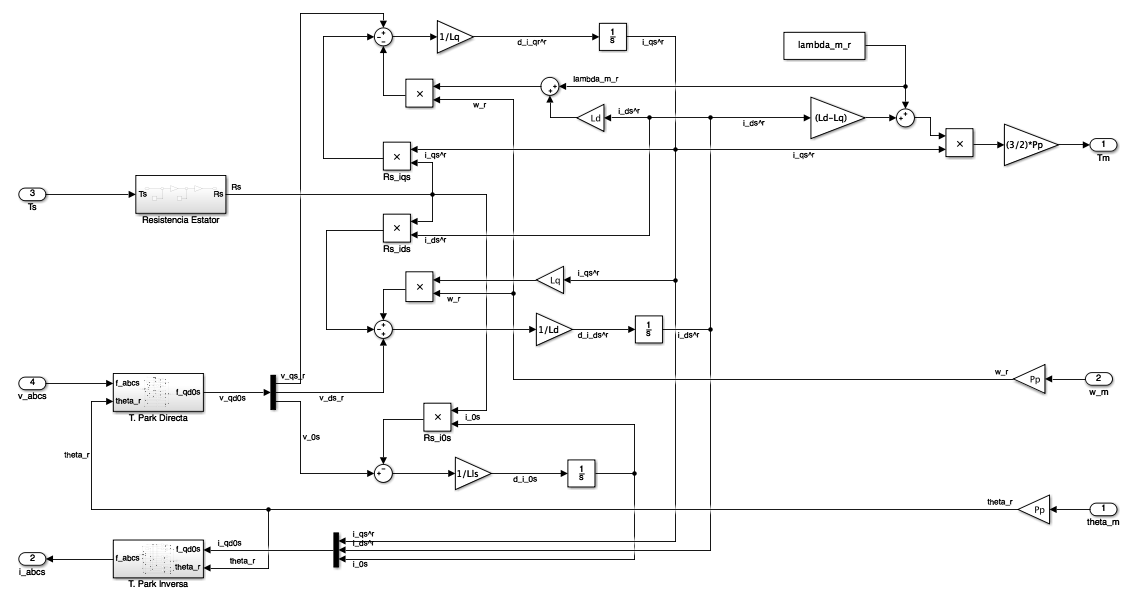
\includegraphics[width=\textwidth]{2_1_2_ModeloElectricoEquivalente.png}
			\caption{\label{fig:ElectricoEquivalente} Diagrama en bloques de la planta completa en \textbf{Simulink} (con transformación de \textbf{Park})}
		\end{figure}

		\item \textbf{Subsistema Térmico:}\vspace{0.3cm}\\
		Para el análisis y modelado térmico de la máquina eléctrica, vamos a considerar sólo pérdidas resistivas por \textbf{Efecto Joule} en el bobinado del estator y despreciar pérdidas magnéticas. La transferencia de calor es por conducción y convección natural, sin ventilación forzada.

		La potencia de pérdidas en coordenadas $abc$ del estator está dada por:
		\begin{equation}
			P_{s\ perd}\left ( t \right )=R_{s}\left ( t \right )\cdot \left ( {i_{as}}^{2}\left ( t \right )+{i_{bs}}^{2}\left ( t \right )+{i_{cs}}^{2}\left ( t \right ) \right )
		\end{equation}
		Y en coordenadas $qd0$ fijas en rotor:
		\begin{equation}
			\label{eqn:potenciaDisipada}
			P_{s\ perd}\left ( t \right )=\frac{3}{2}\cdot R_{s}\left ( t \right )\cdot \left ( {i_{qs}^{r}}^{2}\left ( t \right )+{i_{ds}^{r}}^{2}\left ( t \right )+2\cdot {i_{0s}^{r}}^{2}\left ( t \right ) \right )
		\end{equation}
		Donde hay que tener en cuenta que la resistencia del estator $R_{s}$, varía con la temperatura según la expresión:
		\begin{equation}
			\label{eqn:variacionRs}
			R_{s}\left ( t \right )=R_{sREF}\cdot \left ( 1+\alpha_{Cu}\cdot \left ( {T_{s}}^{\circ}\left ( t \right )-{T_{sREF}}^{\circ} \right ) \right )
		\end{equation}
		El balance térmico entonces, queda dado por la siguiente ecuación:
		\begin{equation}
			\label{eqn:balanceTermico}
			P_{s\ perd}\left ( t \right )=C_{ts}\cdot \frac{\mathrm{d} {T_{s}}^{\circ}\left ( t \right )}{\mathrm{d} t}+\frac{1}{R_{ts-amb}}\cdot \left ( T_{s}^{\circ}\left ( t \right )-T_{amb}^{\circ}\left ( t \right ) \right )
		\end{equation}

		\item \textbf{Dinámica del modelo global NL:}\vspace{0.3cm}\\
		Teniendo en cuenta la ecuación \ref{globalNL:omegaM}; reemplazando \ref{sist:electromagnetico} en \ref{sist:mecanico}; reacomodando las ecuaciones \ref{sist:electrico1}, \ref{sist:electrico2} y \ref{eqn:expresionNula}; reemplazando \ref{eqn:potenciaDisipada} en \ref{eqn:balanceTermico} y reacomodando; y considerando la ecuación \ref{eqn:variacionRs} el modelo dinámico \textbf{global NL} del sistema nos queda:
		
		
		\begin{equation}
			\label{eqn:sistGlobalNL}
			\begin{cases}
				\dot{\theta_{m}}(t)=\omega_{m}(t)
				\\
				\\
				\dot{\omega }_{m}\left ( t \right )=\frac{3}{2}\cdot\frac{P_{p}}{J_{eq}}\cdot [ \lambda_{m}^{r'}+\left ( L_{d}-L_{q} \right )\cdot i_{ds}^{r} (t)]\cdot i_{qs}^{r}(t)-\frac{b_{eq}}{J_{eq}}\cdot\omega_{m}(t)-\frac{T_{eq}(t)}{J_{eq}}
				\\
				\\
				\frac{\mathrm{d} i_{qs}^{r}\left ( t \right )}{\mathrm{d} t}=\frac{v_{qs}^{r}(t)}{L_{q}}-\frac{R_{s}\left ( t \right )}{L_{q}}\cdot i_{qs}^{r}(t)-\frac{P_{p}}{L_{q}}\cdot [ \lambda_{m}^{r'}+L_{d}\cdot i_{ds}^{r}(t) ]\cdot \omega_{m}(t)
				\\
				\\
				\frac{\mathrm{d} i_{ds}^{r}\left ( t \right )}{\mathrm{d} t}=\frac{v_{ds}^{r}(t)}{L_{d}}-\frac{R_{s}\left ( t \right )}{L_{d}}\cdot i_{ds}^{r}(t)+\frac{P_{p}\cdot L_{q}}{L_{d}}\cdot i_{qs}^{r}(t)\cdot \omega_{m}(t)
				\\
				\\
				\frac{\mathrm{d} i_{0s}^{r}\left ( t \right )}{\mathrm{d} t}=\frac{v_{0s}^{r}(t)}{L_{ls}}-\frac{R_{s}\left ( t \right )}{L_{ls}}\cdot i_{0s}^{r}\left ( t \right )
				\\
				\\
				\frac{\mathrm{d} {T_{s}}^{\circ}\left ( t \right )}{\mathrm{d} t}=\frac{\frac{3}{2}\cdot R_{s}\left ( t \right )\cdot \left ( {i_{qs}^{r}}^{2}\left ( t \right )+{i_{ds}^{r}}^{2}\left ( t \right )+2\cdot {i_{0s}^{r}}^{2}\left ( t \right ) \right )-\frac{T_{s}^{\circ}\left ( t \right )-T_{amb}^{\circ}\left ( t \right )}{R_{ts-amb}}}{C_{ts}}
				\\
				\\
				R_{s}\left ( t \right )=R_{sREF}\cdot \left ( 1+\alpha_{Cu}\cdot \left ( {T_{s}}^{\circ}\left ( t \right )-{T_{sREF}}^{\circ} \right ) \right )
			\end{cases}
		\end{equation}
		Este modelo contiene varias \textbf{no linealidades} al contener productos de variables de estado y también al depender varias de esas ecuaciones de $R_{s}$, que a su vez depende de la temperatura ${T_{s}}^{\circ}$ que es una variable de estado que varia en el tiempo $t$.
		\\
		\\
		Este modelo \textbf{NL} puede ser representado mediante diagramas de bloques en \textbf{Simulink} como se observa en la figura \ref{fig:ElectricoEquivalente}.

	\end{itemize}
	%% Esto lo puse porque sino la imagen quedaba mal acomodada, ver si al completar lo primero hace falta o ya no. !!!!!!!!!!!!!!!!!!!!!!!!!!!!!!!!!!!!!!!!!!!!!!!
  

	\item \textbf{Linealización Jacobiana}
    \vspace{0.3cm} 
    \\Primero obtendremos el modelo \textbf{global linealizado con parámetros variables (LPV)}, para $ i_{ds}^{r}\left( t \right ) \neq 0 $ (caso gral.). 
    Un sistema \textbf{no lineal} puede ser representado por:
    \begin{equation}
		\begin{cases}
			\dot{x}\left ( t \right )= f\left ( x\left ( t \right ),u\left ( t \right ),t \right ) \ \ \ ,\ \ \ x\left ( t_{0} \right )=x_{0}
			\\
			y\left ( t \right )= C \cdot x\left ( t \right )
		\end{cases}
    \end{equation}
    donde $f$ es una función vectorial \textbf{NL} de $n\times 1$ elementos que está en función del vector de estados $x$.
    El número $n$ es el orden del sistema y la solución de $x(t)$ representa una curva en el espacio de estado \textbf{(trayectoria de estado)}.
    Asumiendo que cada variable se pueden expresar como
    \begin{equation}
        z\left ( t \right )\equiv Z_{0} + \Delta z\left ( t \right )
    \end{equation}
    donde $Z_{0}$ es una magnitud cuasi-estacionaria de variaciones lentas en el tiempo \textbf{(baja dinámica)} y $\Delta z(t)$ una magnitud pequeña de variación rápida en el tiempo \textbf{(alta dinámica)}.
    El sistema queda expresado por:
    \begin{equation}
        \begin{cases}
            \frac{\mathrm{d} X_{o}\left ( t \right )}{\mathrm{d} t}+
            \frac{\mathrm{d} \Delta x\left ( t \right )}{\mathrm{d} t}
            =
            f\left ( X_{o}\left ( t \right )+\Delta x\left ( t \right ),U_{o}\left ( t \right )+\Delta u\left ( t \right ) \right )
            \ \ \rightarrow \ \ 
            X_{o}\left ( 0 \right )=x_{0}\ \ ;\ \ \ \Delta x\left ( 0 \right )=0
			\\
			\\
			Y_{o}(t)+\Delta y(t)=C\cdot (X_{o}\left ( t \right )+\Delta x\left ( t \right ))
			\ \ \rightarrow \ \ 
			Y_{o}\left ( t \right )=C\cdot X_{o}(t)\ \ ;\ \ \ \Delta y\left ( t \right )=C\cdot \Delta x\left ( t \right )
        \end{cases}
    \end{equation}
	Expresando mediante expansión por series de \textbf{Taylor truncada a 1° orden}, podemos plantear:
	\begin{equation}
		\begin{array}{l}
			\textcolor{red}{f(} X_{o}(t)+\Delta x(t),U_{o}(t)+\Delta u(t) \textcolor{red}{)} \approx \dots
			\\
			\\
			\ \ \ \ 
			\textcolor{red}{f( X_{o}(t),U_{o}(t) )}+
			\left.\begin{matrix}
				\begin{bmatrix}
					\frac{\partial f}{\partial x_{1}} & \dots & \frac{\partial f}{\partial x_{n}}
				\end{bmatrix}
			\end{matrix}\right|_{0}(t)\cdot \Delta x(t)+
			\left.\begin{matrix}
				\begin{bmatrix}
					\frac{\partial f}{\partial u_{1}} & \dots & \frac{\partial f}{\partial u_{n}}
				\end{bmatrix}
			\end{matrix}\right|_{0}(t)\cdot \Delta u(t)
		\end{array}
	\end{equation}
	A continuación vamos a separar el modelo en dos partes, \textbf{Espacio Global de Puntos de Operación + Modelo Dinámico Local de Pequeñas Desviaciones}.
	En el caso de que el punto de operación esté fijo, tendremos un sistema LTI; en cambio si este varía, tendremos un sistema LTV.
	\\
	El espacio global de puntos de operación se obtiene de la solución del sistema de ecuaciones no lineales definido por la ecuación:
	\begin{equation}
		\label{eqn:equilibrioDinamico}
		\frac{\mathrm{d} X_{o}(t)}{\mathrm{d} t}=f(X_{o}(t),U_{o}(t))\approx 0/const
	\end{equation}
	Si aplicamos la ecuación \ref{eqn:equilibrioDinamico} a la ecuación \ref{eqn:sistGlobalNL} de nuestro modelo, obtenemos el siguiente sistema de ecuaciones:
	\begin{equation}
		\label{eqn:equilibrioDinamicoSistema}
		\begin{cases}
			\dot{\Theta}_{mo}(t)=\Omega_{mo}(t)
			\\
			\\
			0=\frac{3}{2} \cdot \frac{ P_{p}}{J_{eq}}\cdot \left [ \lambda_{m}^{r'}+\left ( L_{d}-L_{q} \right )\cdot I_{dso}^{r} \left ( t \right ) \right ] \cdot I_{qso}^{r}\left ( t \right )-\frac{b_{eq}}{J_{eq}}\cdot \Omega_{mo}\left ( t \right )-\frac{T_{eqo}(t)}{J_{eq}}
			\\
			\\
			0=\frac{V_{qso}^{r}(t)}{L_{q}}-\frac{R_{so}(t)}{L_{q}}\cdot I_{qso}^{r}(t)-\frac{P_{p}}{L_{q}}\cdot [ \lambda_{m}^{r'}+L_{d}\cdot I_{dso}^{r}(t) ]\cdot \Omega_{mo}(t)
			\\
			\\
			0=\frac{V_{dso}^{r}(t)}{L_{d}}-\frac{R_{so}\left ( t \right )}{L_{d}}\cdot I_{dso}^{r}(t)+\frac{P_{p}\cdot L_{q}}{L_{d}}\cdot I_{qso}^{r}(t)\cdot \Omega_{mo}(t)
			\\
			\\
			0=\frac{V_{0so}^{r}(t)}{L_{ls}}-\frac{R_{so}\left ( t \right )}{L_{ls}}\cdot I_{0so}^{r}(t)
			\\
			\\
			0=\frac{\frac{3}{2}\cdot R_{so}(t)\cdot \left ( {I_{qso}^{r}}^{2}(t)+{I_{dso}^{r}}^{2}(t)+2\cdot {I_{0so}^{r}}^{2}(t) \right )-\frac{T_{so}^{\circ}\left ( t \right )-T_{amb}^{\circ}\left ( t \right )}{R_{ts-amb}}}{C_{ts}}
			\\
			\\
			R_{so}(t)=R_{sREF}\cdot \left ( 1+\alpha_{Cu}\cdot \left ( {T_{so}}^{\circ}\left ( t \right )-{T_{sREF}}^{\circ} \right ) \right )
		\end{cases}
	\end{equation}
	Este sistema de ecuaciones representa un \textbf{``equilibrio"\  dinámico} cuasi-estacionario del sistema. Por otro lado, alrededor de los puntos de operación nuestro modelo dinámico local de pequeñas desviaciones viene dado por la ecuación:
	\begin{equation}
		\label{eqn:pequeniasDesviaciones}
		\frac{\mathrm{d} \Delta x(t)}{\mathrm{d} x}=
		\begin{bmatrix}
			\left.\begin{matrix}
				\frac{\partial f}{\partial x}
			\end{matrix}\right|_{0}(t)
		\end{bmatrix}\cdot\Delta x(t)+
		\begin{bmatrix}
			\left.\begin{matrix}
				\frac{\partial f}{\partial u}
			\end{matrix}\right|_{0}(t)
		\end{bmatrix}\cdot\Delta u(t)
		\ \ ;\ \ \Delta x(0)=0
	\end{equation}
	Si aplicamos la ecuación \ref{eqn:pequeniasDesviaciones} a la ecuación \ref{eqn:sistGlobalNL} de nuestro modelo, obtenemos el siguiente sistema de ecuaciones del modelo dinámico LPV (pequeñas variaciones locales):
	\newline
	\begin{equation}
		\label{eqn:sistPequeniasDesviaciones}
		\begin{cases}
			\Delta\dot{\theta}_{m}(t)=\Delta\omega_{m}(t)
			\\
			\\
			\Delta\dot{\omega }_{m}(t)=\frac{3 P_{p}}{2 J_{eq}}\cdot \left [[\lambda_{m}^{r'}+\left ( L_{d}-L_{q} \right )\cdot I_{dso}^{r} (t)]\cdot\Delta i_{qs}^{r}(t)+[\left ( L_{d}-L_{q} \right )\cdot I_{qso}^{r}(t)]\cdot\Delta i_{ds}^{r} (t)\right ]\dots \\  \ \ \ \ \ \ \  \  \ \  \ \  \ \ \ \ - \frac{b_{eq}}{J_{eq}}\cdot\Delta\omega_{m}(t)-\frac{\Delta T_{eq}(t)}{J_{eq}}
			\\
			\\
			\frac{\mathrm{d} \Delta i_{qs}^{r}\left ( t \right )}{\mathrm{d} t}=\frac{\Delta v_{qs}^{r}(t)}{L_{q}}-\left [ \frac{R_{so}\left ( t \right )}{L_{q}}\cdot \Delta i_{qs}^{r}(t)+\frac{\Delta R_{s}(t)}{L_{q}}\cdot I_{qso}^{r}(t) \right ]\dots \\ \ \ \ \ \ \ \  \  \ \  \ \  \ \ \ \ -\frac{P_{p}}{L_{q}}\cdot\left [[\lambda_{m}^{r'}+L_{d}\cdot I_{dso}^{r}(t)]\cdot\Delta \omega_{m}(t)+[L_{d}\cdot \Omega_{mo}(t)]\cdot \Delta i_{ds}^{r}(t)\right ]
			\\
			\\
			\frac{\mathrm{d}\Delta i_{ds}^{r}\left ( t \right )}{\mathrm{d} t}=\frac{\Delta v_{ds}^{r}(t)}{L_{d}}-\left [ \frac{R_{so}\left ( t \right )}{L_{d}}\cdot \Delta i_{ds}^{r}(t)+\frac{\Delta R_{s}\left ( t \right )}{L_{d}}\cdot I_{dso}^{r}(t) \right ]\dots \\ \ \ \ \ \ \ \  \  \ \  \ \  \ \ \ \ +\frac{P_{p}\cdot L_{q}}{L_{d}}\cdot\left [  I_{qso}^{r}(t)\cdot \Delta\omega_{m}(t)+\Delta i_{qs}^{r}(t)\cdot \Omega_{mo}(t) \right ]
			\\
			\\
			\frac{\mathrm{d}\Delta i_{0s}^{r}\left ( t \right )}{\mathrm{d} t}=\frac{\Delta v_{0s}^{r}(t)}{L_{ls}}-\left [ \frac{R_{so}\left ( t \right )}{L_{ls}}\cdot \Delta i_{0s}^{r}(t)+\frac{\Delta R_{s}\left ( t \right )}{L_{ls}}\cdot I_{0so}^{r}(t) \right ]
			\\
			\\
			\frac{\mathrm{d} {\Delta T_{s}}^{\circ}\left ( t \right )}{\mathrm{d} t}=\frac{3R_{so}(t)}{C_{ts}}\cdot \left [ I_{qso}^{r} \cdot \Delta i_{qs}^{r}+I_{dso}^{r} \cdot \Delta i_{ds}^{r}+2I_{0so}^{r} \cdot \Delta i_{0s}^{r} \right ]+\frac{3\Delta R_{s}(t)}{2 C_{ts}}\cdot\left [ {I_{qso}^{r}}^{2}+{I_{dso}^{r}}^{2}+2\cdot{I_{0so}^{r}}^{2} \right ]\dots \\ \ \ \ \ \ \ \  \  \ \  \ \  \ \ \ \ -\frac{\left [\Delta T_{s}^{\circ}\left ( t \right )  - \Delta T_{amb}^{\circ}\left ( t \right ) \right ]}{R_{ts-amb}\cdot C_{ts}}
			\\
			\\
			\Delta R_{s}( t )=R_{sREF}\cdot\alpha_{Cu}\cdot {\Delta T_{s}}^{\circ}( t )
		\end{cases}
	\end{equation}
	El modelo global NL dado por la ecuación \ref{eqn:sistGlobalNL}, se puede linealizar por series de Taylor truncadas al primer orden obteniendo 
	un modelo lineal dado por la ec. \ref{eqn:sistPequeniasDesviaciones} alrededor de puntos de operación definidos por la ec. \ref{eqn:equilibrioDinamicoSistema} con estado inicial genérico.

    \item \textbf{Linealización por Realimentación NL}
    \begin{itemize}
    
	\item\textbf{ Modelo simplificado lineal invariante (LTI) equivalente}.
	
	A continuación se presenta el modelo (LTI) en espacio de estado obtenido del modelo NL completo, considerando que la corriente  		$i^{r}_{ds}$ en directo con el campo magnético principal generado por imanes permanentes es nula, la resistencia en los 			devanados del estator es constante con la temperatura, el sistema es equilibrado y simétrico, por lo que  $i^{r}_{0s}=0$ y que  el modelo del subsistema térmico es lineal.\\
	Definimos el vector de estados $X(t)$ (ec.\ref{eq:2.1.2.c.1}), la perturbación $d(t)$ (ec.\ref{eq:2.1.2.c.3}) y el vector de entradas $u(t)$ (ec.\ref{eq:2.1.2.c.2}) :
	\begin{equation}
		X(t)=\begin{bmatrix}
			\theta_{m}(t)\\
			\omega_{m}(t) 
			\\ 
			i^{r}_{qs}(t)\\
			T°_{s}(t)
		\end{bmatrix}
		\label{eq:2.1.2.c.1}
	\end{equation}
		\begin{equation}
		d(t)=\frac{T_{l}(t)}{r} 
		\label{eq:2.1.2.c.3}
	\end{equation}
	
	\begin{equation}
		u(t)=\begin{bmatrix}
			v^{r}_{qs} (t)\\
			d(t)\\
			P_{s perd}(t)\\
			T°_{amb}(t) 
		\end{bmatrix}
		\label{eq:2.1.2.c.2}
	\end{equation}

	Asi el modelo LTI en el espacio de estados es el siguiente  :
	
	\begin{equation}
	\begin{cases}
	\dot{X}(t)=\begin{bmatrix}
	0 & 1 &0 &0\\ 
	0 & -\frac{b_{eq}}{J_{eq}} & \frac{3 P_{p} \lambda^{r'}_{m}}{2 J_{eq}} & 0\\ 
	0  & \frac{- P_{p} \lambda^{r'}_{m}}{ L_{q}} & \frac{-R_{s}}{L_{q}} & 0\\
	0 & 0 & 0 & -\frac{1}{R_{ts-amb} C_{ts}}
	\end{bmatrix}\cdot X(t) + \begin{bmatrix}
	0 &0 &0 &0\\ 
	0 &\frac{-1}{J_{eq}} &0 &0\\ 
	 \frac{1}{L_{q}}&0 &0 & 0\\
	0 & 0 & \frac{1}{C_{ts}} & \frac{1}{R_{ts-amb} C_{ts}}
	\end{bmatrix} 
	\cdot u(t); \\
	X(t_{0})=x_{0}\\ 
	y(t)=[1 \ \ 0 \ \ 0 \ \ 1] \cdot X(t)
	\end{cases}
	\label{eq:2.1.2.c.4}
	\end{equation}
	Es importante notar que con estas restricciones obtenemos un sistema algebraico completamente lineal, la matriz de coeficientes \textbf{A} es constante, además el torque electromagnético (ec. \ref{sist:electromagnetico}) dependerá solamente de $i^{r}_{qs}$ y la tensión inducida en el eje en cuadratura q (ec. \ref{sist:electrico1}) dependerá solamente de $w_{m}$.
	En la figura \ref{fig:diagLTI} se muestra el diagrama de bloques en forma desagregada del sistema (rosado). Como vemos imponiendo la restricción $i^{r}_{ds}=0$ el sistema toma la forma de un motor de corriente continua.
	\begin{figure}[h!]
		\centering
		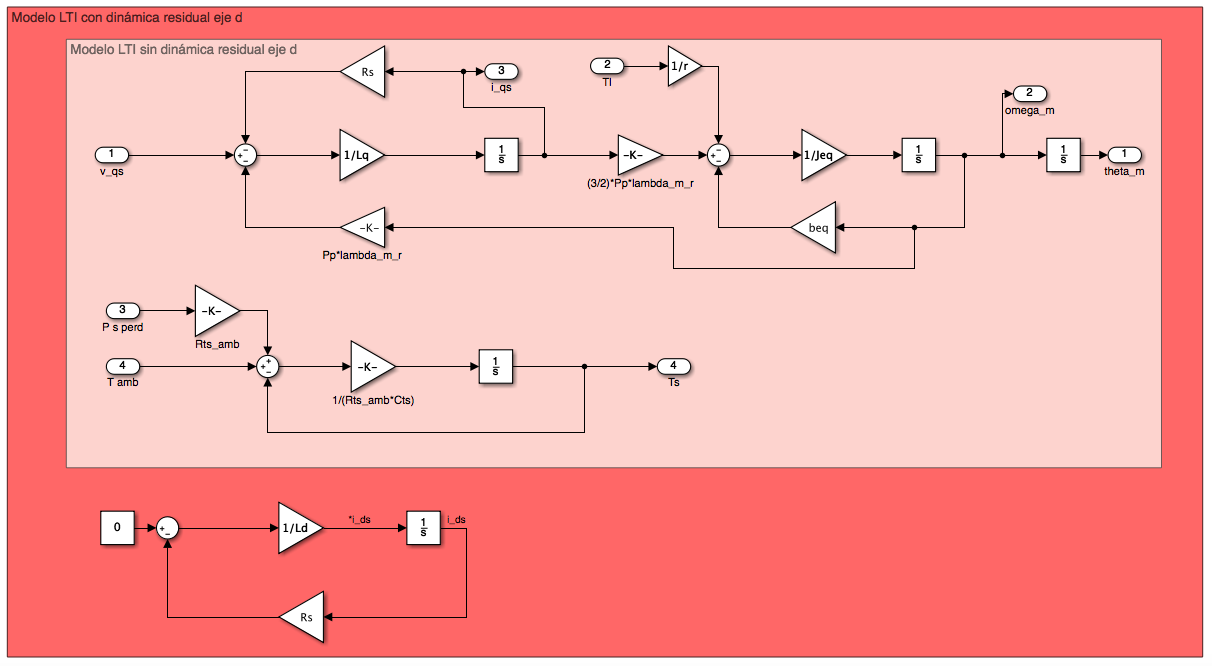
\includegraphics[width=0.9\textwidth]{DiagramabloquesLTI.png}
		\caption{\label{fig:diagLTI} Diagrama de bloques de estado del modelo simplificado lineal invariante (LTI) equivalente en \textbf{Simulink}. Con dinámica residual (rojo) y sin dinámica residual (rosado). }
	\end{figure}

	\item\textbf{ Restricción o Ley de Control mínima}.\\
	Para lograr una $i^{r}_{ds}$ nula y asi obtener el modelo LTI desarrollado en el punto anterior debemos aplicar sobre el eje d la ley de control expresada por la ec. \ref{eq:2.1.2.d.1}.
	\begin{equation}
	v^{r}_{ds}(t)=-L_{q}\cdot i^{r}_{qs}(t)\cdot P_{p}\cdot \omega_{m}(t)\ ; i^{r}_{ds}(t_{0})=0
	\label{eq:2.1.2.d.1}
	\end{equation}
	
	Esta restricción se obtiene al imponer la condición $i^{r}_{ds}\equiv 0$ en la ec.\ref{sist:electrico2}, lo que define una ecuación algebraica que representa una restricción sobre $v^{r}_{ds}(t)$. Asi $v^{r}_{ds}(t)$ deja de ser una variable manipulada. Como podemos ver se ha considerado que la condición inicial de $i^{r}_{ds}$ es nula, ya que si esta no lo fuera tendríamos una dinámica residual de la corriente $i^{r}_{ds}$ lo que provocaría que el modelo no sea lineal en los instantes iniciales, esto lo desarrollaremos en detalle más adelante. Por otro lado para implementar esta ley de control es necesario realimentar a nuestro controlador con las variables de estado $i^{r}_{qs}$ y $\omega_{m}$, y que este genere una consigna de tensiones de fase congruente con dicha restricción. Para ello en el controlador se implementa una transformación directa de Park para así poder trabajar con las tensiones $v^{r}_{qd0s}$, ya que, de la planta sensamos $v_{abcs}$, así generamos nuestras consignas de tensiones $v^{r}_{qd0s}$ y luego mediante una transformación inversa de Park obtenemos las consignas de tensiones de fase $v_{abcs}$, capaces de reproducir dicha restricción, y estas consignas de tensiones se generarán mediante el modulador de tensión, conmutado con modulación de ancho de pulso PWM, en este análisis el modulador de tensión se idealiza considerando solamente las componentes fundamentales, sin armónicos de las ondas de tensión. Esta técnica se denomina \textbf{linealización por realimentación directa no lineal de estado parcial} y obtenemos así el modelo \textbf{NL desacoplado con Ley de control NL}.\\
     En el diagrama de bloques del modelo NL (figura \ref{fig:ElectricoEquivalente}) podemos observar en rojo el desacoplamiento que esta restricción impone.\\
     En la figura \ref{fig:diagrestriccionminima} se puede ver la implementación de esta ley de Control en color rojo dentro del controlador parcial.

	
	\begin{figure}[h!]
	\centering
	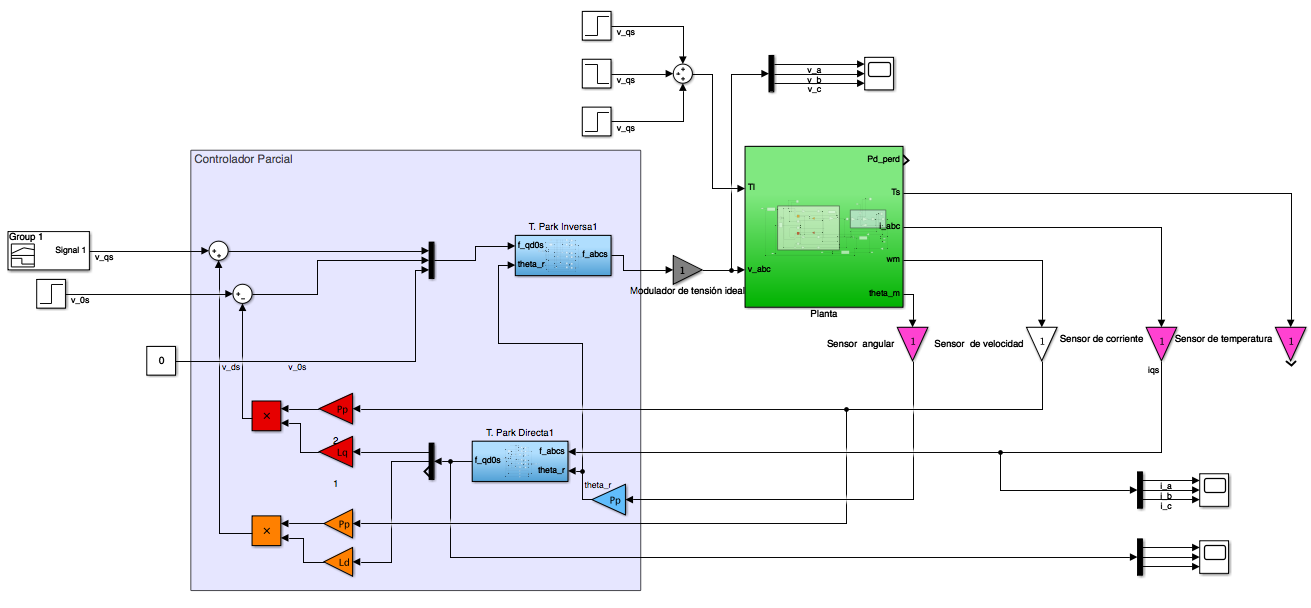
\includegraphics[width=\textwidth]{realimentacionNL.png}
	\caption{\label{fig:diagrestriccionminima} Impelementación controlador parcial con restricción mínima (rojo) y con restricción complementaria (naranja). Planta (verde), sensores(rojo), controlador parcial (celeste).}
	\end{figure}
	
	\item\textbf{Dinámica residual en el eje d}\\
	El modelo de la dinamica residual para $i^{r}_{ds}$ al aplicar la ley de control mínima para el caso de que $i^{r}_{ds}(0)\neq 0$ se muestra en la ec.\ref{eq:2.1.2.e.1} y su ecuación de transeferencia esta dada por la ec.\ref{eq:2.1.2.e.2}.
	\begin{equation}
	\frac{di^{r}_{ds}}{dt}=\frac{R_{s}}{L_{d}}\ i^{r}_{ds}(t)
	\label{eq:2.1.2.e.1}
	\end{equation}
	\begin{equation}
	\frac{I^{r}_{ds}(s)}{E(s)}=\frac{1}{s+\frac{R_{s}}{L_{d}}}
	\label{eq:2.1.2.e.2}
	\end{equation}
	
	Vemos que la dinámica residual tiene la forma de una ecuación diferencial monótona descendiente con un cero en $s=-154.55$, si consideramos a $Rs$ constante e igual a 1.02. Por lo que podemos concluir que ante un estado inicial distinto de cero la corriente en el eje d va a tender rápidamente a cero.
	Si incorporamos esta dinámica residual a nuestro modelo LTI (ec.\ref{eq:2.1.2.c.4}) obtenemos:
		\begin{equation}
		X(t)=\begin{bmatrix}
			\theta_{m}(t)\\
			\omega_{m}(t) 
			\\ 
			i^{r}_{qs}(t)\\
			T°_{s}(t)\\
		i^{r}_{ds}
		\end{bmatrix}
		\label{eq:2.1.2.e.3}
	\end{equation}

	\begin{equation}
	\begin{cases}
	\dot{X}(t)=\begin{bmatrix}
	0 & 1 &0 &0&0\\ 
	0 & -\frac{b_{eq}}{J_{eq}} & \frac{3 P_{p} \lambda^{r'}_{m}}{2 J_{eq}} & 0&0\\ 
	0  & \frac{- P_{p} \lambda^{r'}_{m}}{ L_{q}} & \frac{-R_{s}}{L_{q}} & 0&0\\
	0 & 0 & 0 & -\frac{1}{R_{ts-amb} C_{ts}}&0\\
	0&0&0&0&\frac{R_{s}}{L_{d}}
	\end{bmatrix}\cdot X(t) + \begin{bmatrix}
	0 &0 &0 &0\\ 
	0 &\frac{-1}{J_{eq}} &0 &0\\ 
	 \frac{1}{L_{q}}&0 &0 & 0\\
	0 & 0 & \frac{1}{C_{ts}} & \frac{1}{R_{ts-amb} C_{ts}}\\
	0 &0 &0 &0
	\end{bmatrix} 
	\cdot u(t); \\
	X(t_{0})=x_{0}\\ 
	y(t)=[1 \ \ 0 \ \ 0 \ \ 0 \ \ 0]\cdot \ X(t)
	\end{cases}
	\label{eq:2.1.2.e.4}
	\end{equation}
	

	

	Donde vemos que ahora nuestro vector de estado (ec.\ref{eq:2.1.2.e.3}) tiene un estado más y las entradas son las definidas por la ec.\ref{eq:2.1.2.c.2}. Como podemos ver, ahora $i^{r}_{ds}$ puede ser distinta de cero, sin embargo no se ha considerado el \textbf{acoplamiento residual NL con el eje q} dado por la ec. \ref{eq:2.1.2.e.5} y esto se debe a que como comentamos mas arriba la dinámica residual de este eje es monótona descendiente por lo que rápidamente $i^{r}_{ds}$ decae a cero, por ende, en régimen forzado esta no va a tener influencia sobre el \textbf{eje q}.
	
	\begin{equation}
	v^{r*}_{qs}(t)=L_{d}. i^{r}_{ds}(t).P_{p}.\omega_{m}(t)
	\label{eq:2.1.2.e.5}
	\end{equation}
	
	En la figura \ref{fig:diagLTI} se puede apreciar el modelo LTI considerando la dinámica residual del eje d (rojo).
	
	   \item\textbf{Ley de Control complementaria mínima en el eje q}.\\
	    Para eliminar completamente este acoplamiento residual NL aún en régimen natural y obtener un modelo equivalente 				completamente lineal, independiente del estado inicial de $i^{r}_{ds}$ se debe realimentar al sistema con la ley de control 			dada por la ec.\ref{eq:2.1.2.e.5}. En la figura \ref{fig:diagrestriccionminima} se puede apreciar el controlador parcial con la implementación de esta restricción en color naranja, obteniendo asi el modelo \textbf{LTI equivalente aumentado} el cual aplica la ley de control mínima en el eje d y la ley de control complementaria en el eje q.\\
	     En el diagrama de bloques del modelo NL (figura \ref{fig:ElectricoEquivalente})  podemos observar en naranja el desacoplamiento que estarealimentación produce.\\
	\end{itemize}
	
	 \item \textbf{Comparación del modelo dinámico LTI equivalente aumentado vs. el modelo LPV forzando $I^{r}_{ds_{0}} \equiv 0$}.\\
	 Si forzamos $\Delta i^{r}_{ds} \equiv 0$ para lo cual  $\Delta v^{r}_{ds}(t)=-\frac{P_{p}\cdot L_{q}}{L_{d}}\cdot\left [  I_{qso}^{r}(t)\cdot \Delta\omega_{m}(t)+\Delta i_{qs}^{r}(t)\cdot \Omega_{mo}(t) \right ]$, consideramos $R_{s}$ constante y el modelo del subsistema térmico lineal, el modelo LPV se caracteriza por la ecuación \ref{eq:2.1.2.f.1}, donde no se ha incorporado el vector de entradas por una cuestión de espacio, además no es relevante para el análisis.
	 
	 \begin{equation}
		\begin{bmatrix}
	\Delta \dot{\theta}_{m}(t)\\
	\Delta \dot{\omega}_{m}(t)
	\\ 
	\frac{d \Delta i^{r}_{qs}(t)}{dt}\\
	\Delta \dot{T}_{s}(t)\\
	\end{bmatrix}
	=
	\begin{bmatrix}
		0 & 1 &0 &0  \\ 
		0 & -\frac{b_{eq}}{J_{eq}} & \frac{3 P_{p}}{2 J_{eq}}[ \lambda^{r'}_{m}+\left ( L_{d}-L_{q} \right )\cdot I_{dso}^{r} (t)]&0 \\ 
		0  & \frac{- P_{p} }{ L_{q}} [\lambda^{r'}_{m}+L_{d}\cdot I^{r}_{ds0}(t)]& \frac{-R_{s}}{L_{q}}&0\\
		0 & 0 & 0 & -\frac{1}{R_{ts-amb} C_{ts}}\\
		\end{bmatrix} 
	\begin{bmatrix}
	\Delta \theta_{m}(t)\\
	\Delta \omega_{m}(t)
	\\ 
	\Delta i^{r}_{qs}(t)\\
	\Delta T_{s}(t)
	\end{bmatrix}
	\label{eq:2.1.2.f.1}
	\end{equation}
	
	Aplicando esta restricciones y forzando $I^{r}_{ds0} \equiv 0$ , vemos que las matrices del modelo LPV ahora no varían con el tiempo por lo que tenemos un modelo LTI en las cercanías del punto de operación, además podemos observar que las matrices son iguales a las del \textbf{modelo LTI equivalente aumentado} por lo que podriamos decir que este último es un caso particular  del \textbf{modelo dinámico global LPV} obtenido anteriormente. Como se podrá observa en estas ecuaciones no aparece la \textbf{dinámica residual del eje d} ante $i^{r}_{ds}(0)\neq 0$ ni tampoco el \textbf{acoplamiento residual NL en eje q} y esto se debe a que al imponer $I^{r}_{ds_{0}} \equiv 0$ estamos imponiendo indirectamente $i^{r}_{ds}(0)= 0$ ya que al realizar la linealización Jacobiana se le asigna todo el estado incial de las variables de estado a los puntos de operación. \\
	Evaluaremos el comportamiento del sistema para distintos puntos de operación $I^{r}_{ds_{0}}\neq 0$. Por la ecuación del torque electromacnético (ec. \ref{sist:electromagnetico}) y la ecuación \ref{eq:2.1.2.f.1} y recordando que estamos trabajando con una máquina de polos salientes, por lo que $L_{d}$ > $L_{q}$ , se puden debucir tres casos:
	
	\begin{enumerate}
	\item $I^{r}_{ds0}(t)=0$:  el flujo concatenado esta afectado únicamente por los imanes permanentes.
	\item $I^{r}_{ds0}(t)>0$: reforzamiento del campo principal, se logra un mayor torque a costa de menor velocidad
	\item $I^{r}_{ds0}(t)<0$: debilitamiento del campo principal, se logra una mayor velocidad a costa de menor torque
	\end{enumerate}
	Vemos que cuando $I^{r}_{ds0}(t)\neq 0$ se produce una migración de los parámetros de la matriz A que influyen sobre $\omega_{m}$ (velocidad) y $i^{r}_{qs}$ (Torque).
	Si se considera a la máquina como un sistema de potencia constante, fálcimente se puede debucir porque estos cambios en el torque afectan a la velocidad.
	\item \textbf{Función de Transferencia}.
	
	Se desarrollará la función de transferencia para el modelo LTI equivalente aumentado, desde ambas entradas $v^{r}_{qs}(t)$ y $T_{l}$ hacia la salida $\omega_{m}(t)$.\\
	Para obtener esta función partimos de la ecuación \ref{eqn:sistGlobalNL} y le aplicamos la transformada de Laplace a las ecuaciones que representan a $i^{r}_{qs}$ y a $\omega_{m}$ obteniendo:
	\begin{equation}
	i^{r}_{qs}(s).s.L_{q}=V_{qs}(s)-R_{s}.i^{r}_{qs}(s)-\lambda^{r'}_{m}.P_{p}\omega_{m}(s)
	\label{eq:2.1.2.ff.1}
	\end{equation}
	\begin{equation}
	J_{eq}.s.\omega_{m}(s)=\frac{3}{2}.P_{p}.\lambda^{r'}_{m}.i^{r}_{qs}(s)-b_{eq}.\omega_{m}(s)-T_{leq}(s)
	\label{eq:2.1.2.ff.2}
	\end{equation}
	
Despejando $i^{r}_{qs}(s)$ de la ec.\ref{eq:2.1.2.ff.1}, reemplazando en la ec.\ref{eq:2.1.2.ff.2} y reordenando:

\begin{eqnarray}
	\theta_{m}(s)=\frac{\frac{3}{2}P_{p}\lambda^{r'}_{m}}{J_{eq}L_{q}s^{2}+(R_{s}J_{eq}+L_{q}b_{eq})s + \frac{3}{2}P_{p}^{2}\lambda ^{r'2}_{m}+R_{s}b_{eq}} V_{qs}(s) \nonumber\\
	- \frac{L_{s}+R_{s}}{J_{eq}L_{q}s^{2}+(R_{s}J_{eq}+L_{q}b_{eq})s + \frac{3}{2}P_{p}^{2}\lambda ^{r'2}_{m}+R_{s}b_{eq}} T_{leq}(s)
	\label{eq:2.1.2.ff.3}
	\end{eqnarray}
De donde se obtienen las dos funciones de transferencia:
\begin{equation}
	G_{V_{qs}}(s)=\frac{\theta_{m}(s)}{V_{qs}(s)}=\frac{\frac{3}{2}P_{p}\lambda^{r'}_{m}}{J_{eq}L_{q}s^{2}+(R_{s}J_{eq}+L_{q}b_{eq})s + \frac{3}{2}P_{p}^{2}\lambda ^{r'2}_{m}+R_{s}b_{eq}}
	\label{eq:2.1.2.ff.4}
	\end{equation}
	\begin{equation}
	G_{T_{leq}}(s)=\frac{\theta_{m}(s)}{T_{leq}(s)}=\frac{L_{s}+R_{s}}{J_{eq}L_{q}s^{2}+(R_{s}J_{eq}+L_{q}b_{eq})s + \frac{3}{2}P_{p}^{2}\lambda ^{r'2}_{m}+R_{s}b_{eq}}
	\label{eq:2.1.2.ff.5}
	\end{equation} 
\end{enumerate}

Siguiendo el mismo procedimiento se puede obtener las funciones de transferencias dedes las entradas $v^{r}_{qs}(t)$ y $T_{l}$ hacia la salida $i^{r}_{qs}$.\\


\subsubsection{Análisis de Estabilidad a lazo abierto para el modelo LTI equivalente aumentado}

\begin{itemize} 
\item \textbf{Polos y ceros del sistema:}

Para el cálculo de los polos y ceros se tomaron $R_{s}=1.02$ y valores nominales de los parámetros de carga.\\
El sistema tiene un único cero dado por la entrada $T_{leq}$

	\begin{equation}
	Lq . s + R_{s}=0; \ s=-\frac{R_{s}}{L_{q}} = -175.86 \frac{rad}{s}
	\label{eq:2.1.2.g.1}
	\end{equation}
	
Los polos del sistema se obtienen mediante el polinomio característica (ec. \ref{eq:2.1.2.g.2} )

	\begin{equation}
	s.[J_{eq}L_{q}s^{2}+(R_{s}J_{eq}+L_{q}b_{eq})s + \frac{3}{2}P_{p}^{2}\lambda ^{r'2}_{m}+R_{s}b_{eq}]
	\label{eq:2.1.2.g.2}
	\end{equation}
	
De donde facilmente se obtiene:\\
$s_{1}=0$\\

Para calcular los otros polos utilizamos un programa de cálculo como Matlab y asi obtenemos:\\
$s_{2}=-89.26 + 301.57 i$\\
$s_{2}=-89.26 - 301.57 i$

Y para calcular la frecuencia natural y el coeficiente de amortiguamiento se obtuvo de la ec. \ref{eq:2.1.2.g.2} la siguiente ecuación :

	\begin{equation}
	s^{2}+\frac{(R_{s}J_{eq}+L_{q}b_{eq})}{J_{eq}L_{q}}s +\frac{\frac{ \frac{3}{2}P_{p}^{2}\lambda ^{r'2}_{m}}{J_{eq}L_{q}}+R_{s}b_{eq}}{J_{eq}L_{q}}
	\label{eq:2.1.2.g.3}
	\end{equation}
	
y se comparó esta con la ec. \ref{eq:2.1.2.g.4} que se encuentra en función de $\xi$ y $\omega_{n}$.
	\begin{equation}
	s^{2}+2\xi \omega_{n} s + \omega_{n}^2 
	\label{eq:2.1.2.g.4}
	\end{equation}

Por lo tanto se deduce que:\\
$\omega_{n}^2 =\frac{\frac{ \frac{3}{2}P_{p}^{2}\lambda ^{r'2}_{m}}{J_{eq}L_{q}}+R_{s}b_{eq}}{J_{eq}L_{q}}$ \ ; $\omega_{n}=314.5 \frac{rad}{s}$\\
$2\xi \omega_{n}=\frac{(R_{s}J_{eq}+L_{q}b_{eq})}{J_{eq}L_{q}}$ \ ; $\xi=0.2838$

Se puede apreciar que estamos en presencia de un sistema subamortiguado  y que el sistema estable ya que todos los polos tienen parte real negativa.\\

En la figura \ref{fig:polos} se puede observa los polos en el plano imaginario.

	\begin{figure}[h!]
	\centering
	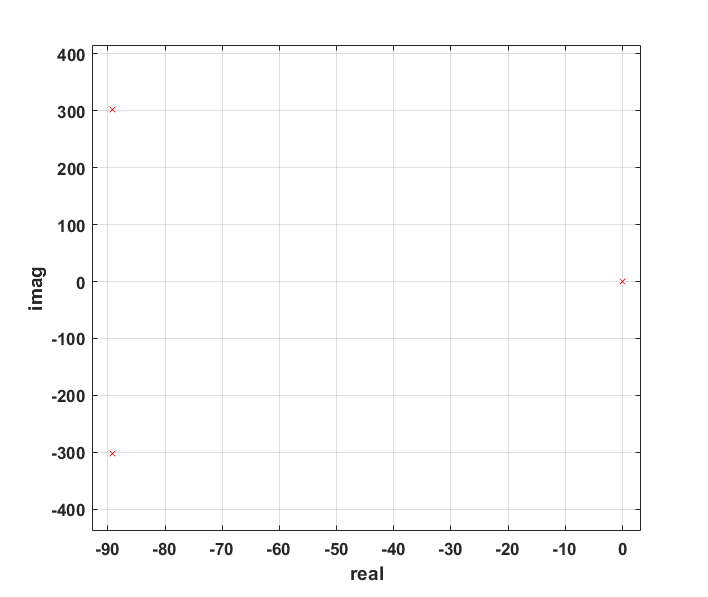
\includegraphics[width=0.5\textwidth]{polos.png}
	\caption{\label{fig:polos}  }
	\end{figure}


Es importante aclarar que al cálcular los autovalores a partir de la función de transferencia del sistema no se ha tenido en cuenta el polo de la dinámica residual calculado anteriormente (ec. \ref{eq:2.1.2.e.2}), pero si hubiesemos tomado los autovalores de A (\ref{eq:2.1.2.e.4}) este polo aparecería. 

\item \textbf{Migración de propiedades:}
Se hace necesario evaluar la estabilidad del sistema ante la variación de los parámetros de carga, ya que como sabemos el robot presenta dinámica no lineal acoplada y se considera como aproximación la dinámica de carga `vista' desde el eje de la articualción hombro, ausmiendo variación de sus parámetros equivalentes. En la figura \ref{fig:varpolos} se observa como cambian los polos del sistema cuando se varían estos parámetros dentro de sus límites de incertidumbre.
	\begin{figure}[h!]
	\centering
	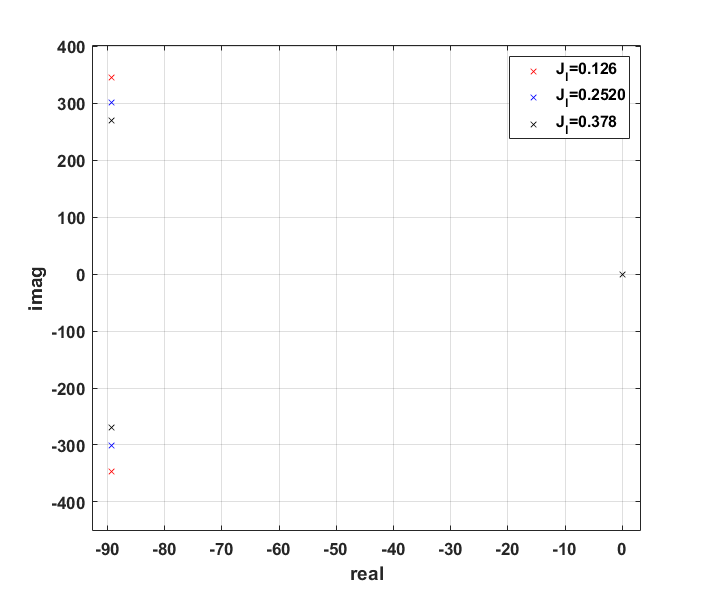
\includegraphics[width=0.5\textwidth]{varpolos.png}
	\caption{\label{fig:varpolos} Migración de polos con variación de $J_{l}$.}
	\end{figure}
	
	Se puedo observar como el aumento de $J_{l}$ provoca una pequeña disminución de la parte real y una mayor de la parte imaginaria del polo y se puede concluir que si los limites de incertidumbre son correctos el sistema va a permanecer estable. Por otra lado el la figura \ref{varpolosbl} se puede ver la variación de estos con respecto a $b_{l}$ y se puede concluir que la variación de este parámetro dentro de sus límites de incertidumbre prácticamente no afecta al sistema.
	
	\begin{figure}[h!]
	\centering
	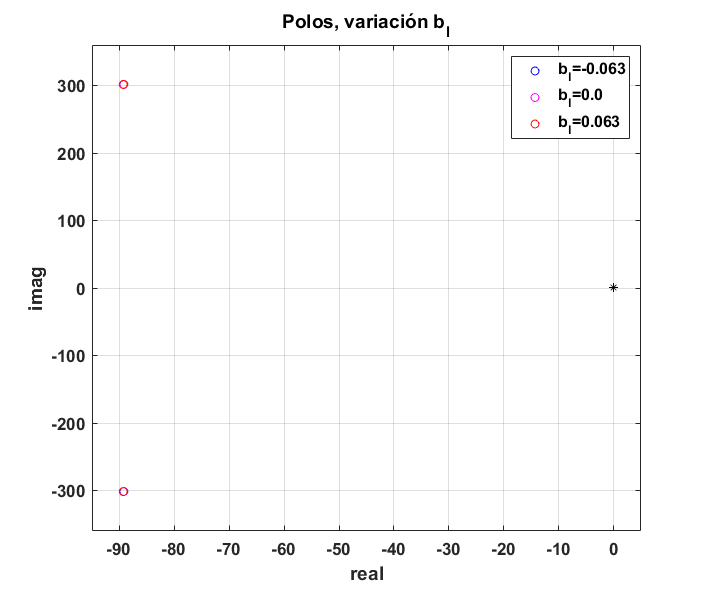
\includegraphics[width=0.5\textwidth]{varpolosbl.png}
	\caption{\label{fig:varpolosbl} Migración de polos con variación de $b_{l}$.}
	\end{figure}
	

\end{itemize}
\subsubsection{Análisis de Observabilidad completa de estado para el modelo LTI equivalente aumentado}
Se cálculo la observabilidad del modelo LTI (ec .\ref{eq:2.1.2.e.4}) mediante el criterio de Kalman (ec.\ref{eq:2.1.2.k.1}) utilizando para esto Matlab.
	\begin{equation}
	Rango \ de\  O=
	\begin{bmatrix}
	
		C\\ 
		C.A\\ 
		...\\ 
		C.A^{n-1}=n
		\end{bmatrix}
	\label{eq:2.1.2.k.1}
	\end{equation}
	
	Donde:
	
		\begin{equation}
		A=\begin{bmatrix}
	0 & 1 &0 &0 \\ 
	0 & -\frac{b_{eq}}{J_{eq}} & \frac{3 P_{p} \lambda^{r'}_{m}}{2 J_{eq}} & 0 \\ 
	0  & \frac{- P_{p} \lambda^{r'}_{m}}{ L_{q}} & \frac{-R_{s}}{L_{q}}&0\\
	0&0&0&\frac{R_{s}}{L_{d}}
	\end{bmatrix}
	\label{eq:2.1.2.k.2}
	\end{equation}
	\begin{equation}
		C=[1 \ \ 0 \ \ 0 \ \ 0 ] 
	\label{eq:2.1.2.k.3}
	\end{equation}
	
Según el criterio de Kalman para que el sistema de la matriz $O$ tiene que ser igual a la cantidad $n$ de estado. Al calcular la observabilidad desde $\theta_{m}(t)$ en base a la ec.\ref{eq:2.1.2.e.4} obtenemos que el rango de esta matriz es 3, por lo que el sistema no es observable, esto se debe a que $i^{r}_{ds}$ no es un estado observable desde $\theta_{m}(t)$, como se puede apreciar en la ec.\ref{eq:2.1.2.e.4} este estado no posee entradas ni salidas. Otro sería el caso si se calculara la observabilidad a partir de la ec. \ref{eq:2.1.2.c.4} también desde $\theta_{m}(t)$ en donde obtendemos que el sistema es completamente observable.

Otra alternativa es medir la observabilidad desde $\omega_{m}$ en donde obtenemos que esta se degrada aún más, ya que además de $i^{r}_{ds}$, $\theta_{m}(t)$ tampoco es observable desde esta. 

\subsubsection{Análisis de Controlabilidad completa de estado para el modelo LTI equivalente aumentado}
Se procedió a calcular la controlabilidad del modelo LTI ec.\ref{eq:2.1.2.e.4} apartir del criterio de Kalman (ec. \ref{eq:2.1.2.l.1}).

	\begin{equation}
		Rango \ de \ C=[B \ A.B \ ... \ A^{n-1}.B]= n
	\label{eq:2.1.2.l.1}
	\end{equation}
	Donde A es la definida en la ec.\ref{eq:2.1.2.k.3} y B es :
	\begin{equation}
		B= \begin{bmatrix}
	0 &0 \\ 
	0 &\frac{-1}{J_{eq}} \\ 
	 \frac{1}{L_{q}}&0 \\
	 0&0
	\end{bmatrix}
	\label{eq:2.1.2.l.2}
	\end{equation}
	
Se concluye que el sistema no es completamente controlable desde la entrada manipulada $v^{r}_{qs}(t)$ dado que el rango de $C$ es 3, esto se debe a que el estado $i^{r}_{ds}$ no es controlable desde $v^{r}_{qs}(t)$, ya que como dijimos anteriormente este un estado aislado del sistema. Para controlador este estado se debería agragar la entrada $v^{r}_{ds}(t)$ volviendo al sistema completamente controlable.

\subsubsection{Simulación dinámica en DT, comparando el modelo NL completo desacoplado con Ley de control
NL vs LTI equivalente aumentado}
\begin{itemize}

\item \textbf{Respuesta del estado interno a pulso de consigna de tensión de estator en eje q, superpuesto con doble pulso de torque de carga.}
A continuación se presentan las respuestas del sistema.
	\begin{figure}[h!]
	\centering
	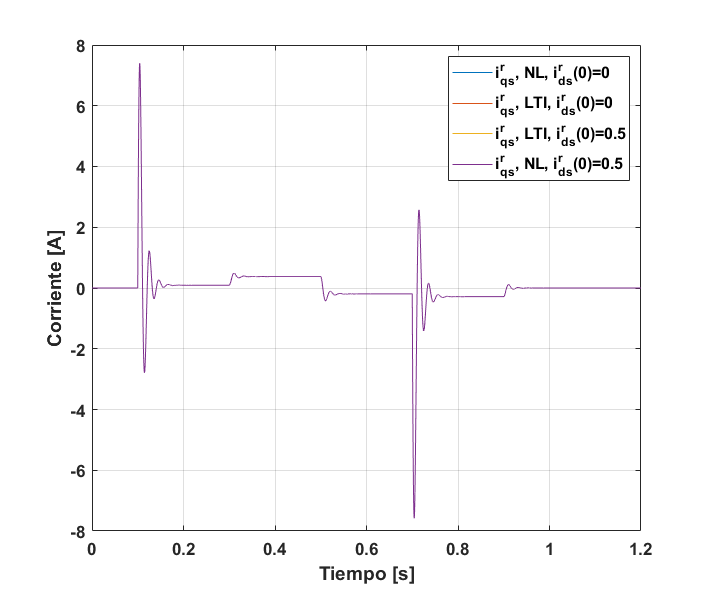
\includegraphics[width=0.7\textwidth]{iq_LTIvsNL.png}
	\caption{\label{fig:iq_LTIvsNL} $i^{r}_{qs}$ vs $t$.}
	\end{figure}
	
	En la figura \ref{fig:iq_LTIvsNL} se puede observar que la corriente establecida en el eje q es igual para ambos modelos, tanto cuando $i^{r}_{s}(0)=0$ como cuando $i^{r}_{ds}(0)=0.5$ esto se debe a que como puede verse en la figura \ref{fig:ids} decrece rápidamente a cero antes que se establezca la consigna $v^{r}_{qs}$ por lo que al estar la máquina estática esta no tiene efecto alguno sobre el sistema y por lo tanto no se produce acoplamiento de esta sobre el eje q ni tiene efecto sobre el torque, es decir, que esta corriente inicial solamente se va a discipar en el devanado del estator. Es por esto que las demás gráficas solamente se graficaron para el modelo NL, ya que presentan el mismo compartamiento para el modelo LTI para la entrada dada como consigna independientemente de $i^{r}_{ds}(0)$.
		\begin{figure}[h!]
	\centering
	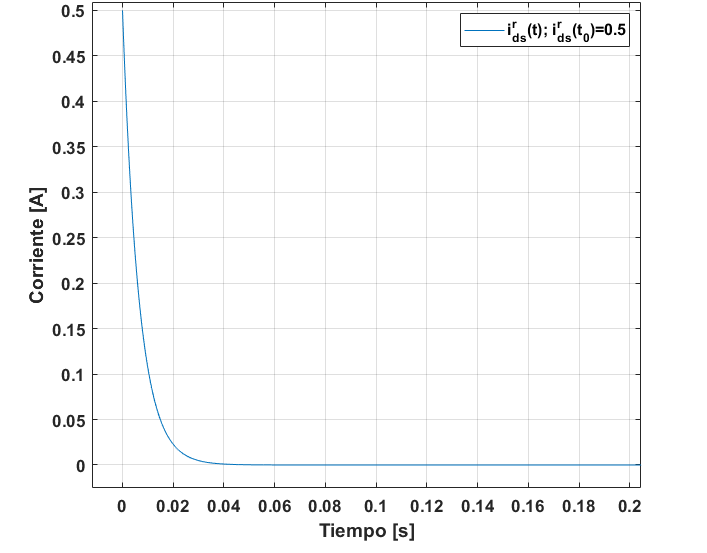
\includegraphics[width=0.7\textwidth]{ids.png}
	\caption{\label{fig:ids} $i^{r}_{ds}$vs t.}
	\end{figure}

	\begin{figure}[h!]
	\centering
	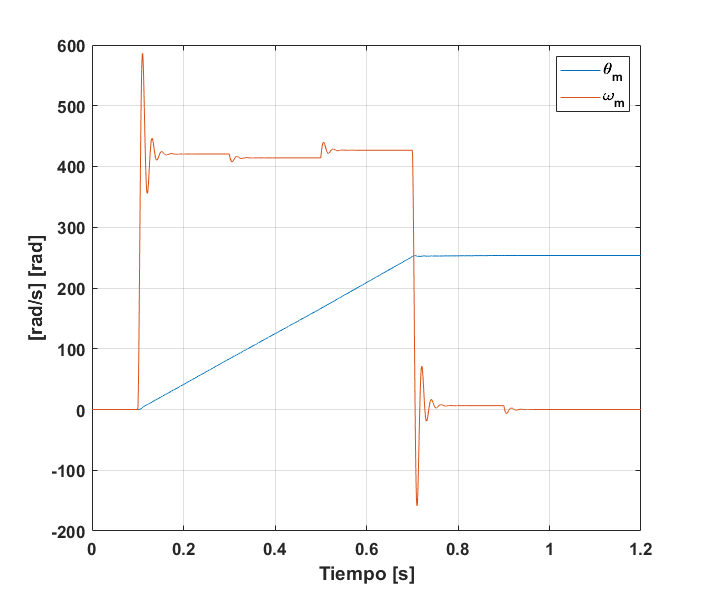
\includegraphics[width=0.7\textwidth]{theta_m.png}
	\caption{\label{fig:theta_m} $\omega_{m}$ vs $t$ y $\theta_{m}$ vs $t$.}
	\end{figure}
	\begin{figure}[h!]
	\centering
	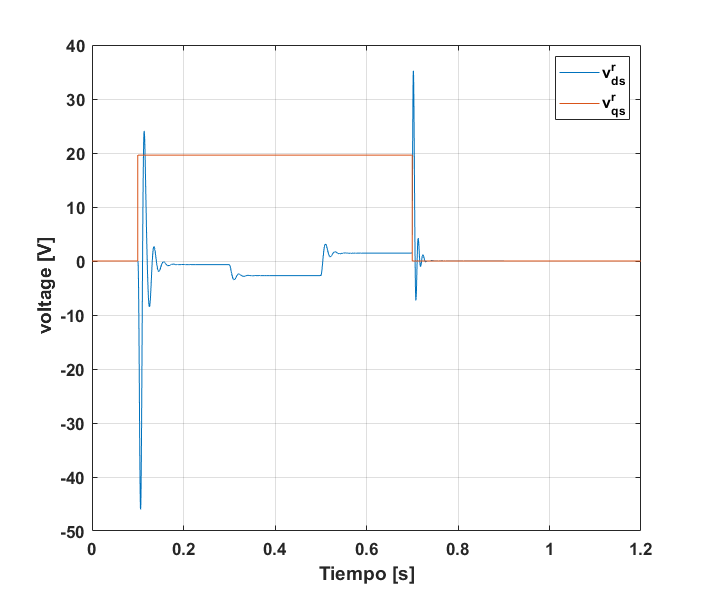
\includegraphics[width=0.7\textwidth]{vd_vq.png}
	\caption{\label{fig:vd_vq} $v^{r}_{ds}$ y $v^{r}_{qs}$.}
	\end{figure}
	\begin{figure}[h!]
	\centering
	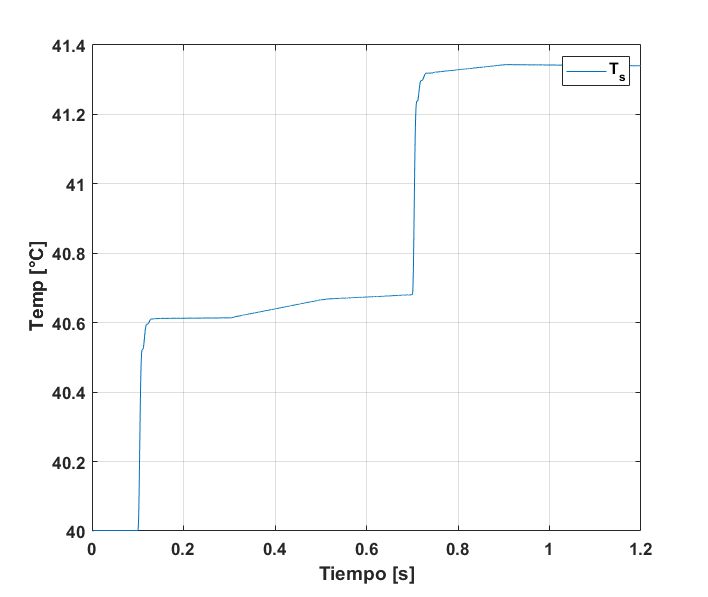
\includegraphics[width=0.7\textwidth]{temperatura.png}
	\caption{\label{fig:temperatura} Temperatura vs t.}
	\end{figure}
	Producto del forzamiento de $i^{r}_{ds}=0$ podemos ver que el sistema se comporta como un motor de CC, ya que la velocidad del motor depende de manera proporcional al voltage de entrada y inversalmente proporcional al torque de carga esto se puede ver claramente observando la figura \ref{fig:theta_m} y la figura\ref{fig:vd_vq}, vemos que luego de afectar con el escalón $v^{r}_{qs}$ la velocidad después de un transtorio se establece constante, lo mismo ocurre en $t=0.3$ cuando se afecta al sistema con un escalón $T_{l}$ provocando una disminución de la velocidad. También hay que notar el excesivo sobrepico en $i^{r}_{qs}$ producto de la consigna de tensión lo que indica que no es buena práctica afectar al sistema con este tipo de entradas, también hay que notar el aumento de la corriente por la entrada de torque dado que el sistema necesitará mayor torque motor para contrarrestar este. \\
	Es importante resaltar como la temperatura (figura \ref{fig:temperatura}) aumenta cada vez que se tiene un pico grande de corriente esto se debe a que esta depende de manera cuadrática de las corrientes.
	Otro punto importante a notar es la gran acción de control $v^{r}_{ds}$ que se realiza para mantener $i^{r}_{ds}=0$ durante el transitorio del sistema.
	 Como se puede ver en las figura \ref{fig:corriente} los sobrepicos en el transitorio vistos en $i^{r}_{qs}$ se corresponden con los sobrepicos en las corrientes de fases y luego de estos transitorios estas convergen a tres ondas sinusoidales desfasadas 120° eléctricos de igual magnitud adoptando una frecuencia tal que $\frac{f_{e}.2\pi}{P_{p}}=\omega_{mestable}$, también se puede observar que cuando $i^{r}_{qs}$ aumenta en magnitud estas también lo hacen y viceversa. El mismo comportamiento se puede observar para las tensiones de fase en la figura \ref{fig:v}.
	\begin{figure}[h!]
	\centering
	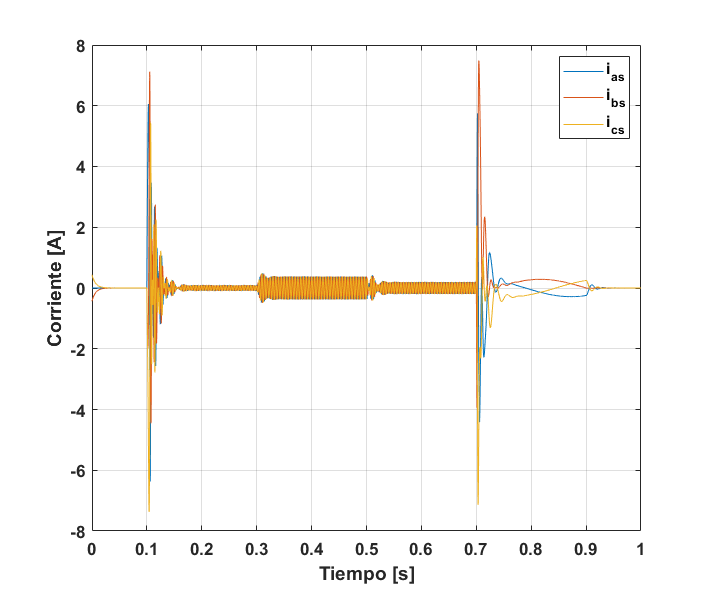
\includegraphics[width=0.7\textwidth]{corriente.png}
	\caption{\label{fig:corriente} Corrientes de fase $i_{abcs}$.}
	\end{figure}
	Partiendo de la transformación inversa de ParK y tomando $i^{r}_{ds}(t) \equiv 0$ , $i^{r}_{0s}(t)=0$ y $v^{r}_{0s}(t)$ podemos obtener analíticamente la forma de la tensión y corrientes $abcs$.\\
	
	$i_{as}(t)=cos(\theta_{r}(t)).i^{r}_{qs}(t)$\\
	$i_{bs}(t)=cos(\theta_{r}(t)-\frac{2}{3}\pi).i^{r}_{qs}(t)$\\
	$i_{cs}(t)=cos(\theta_{r}(t)+\frac{2}{3}\pi).i^{r}_{qs}(t)$\\
	$v_{as}(t)=cos(\theta_{r}(t)).v^{r}_{qs}(t)$ - $ sin(\theta_{r}(t)). v^{r}_{qs}(t)$\\
	$v_{bs}(t)=cos(\theta_{r}(t)-\frac{2}{3}\pi).v^{r}_{qs}(t)$-$sin(\theta_{r}(t)-\frac{2}{3}\pi). v^{r}_{qs}(t)$\\
	$v_{cs}(t)=cos(\theta_{r}(t)+\frac{2}{3}\pi).v^{r}_{qs}(t)$-$sin(\theta_{r}(t)+\frac{2}{3}\pi). v^{r}_{qs}(t)$\\
	
	Como se puede ver las corrientes y tensiones de fase estatóricas siempre van a estar desfasadas 120° eléctricos y simétrico, y para el caso planteado la amplitud de las corrientes dependerá únicamente de $i^{r}_{qs}(t)$.
	\begin{figure}[h!]
	\centering
	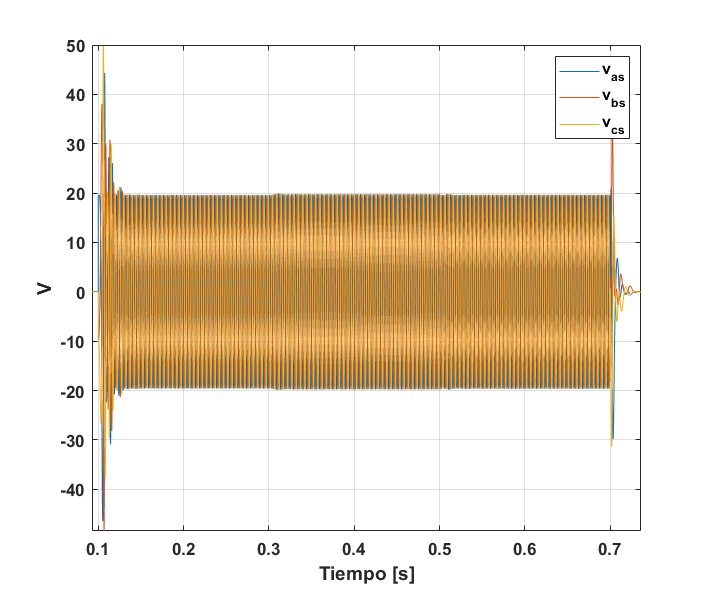
\includegraphics[width=0.7\textwidth]{v.png}
	\caption{\label{fig:v} Tensiones de fase $v_{abcs}$.}
	\end{figure}
	
	En la figura \ref{fig:T vs velocidad} se presenta la curva paramétrica torque vs velocidad con la cual es posible evaluar los cuadrantes de operación del sistema. En primer lugar se debe observar como el motor parte del equilibrio estacionario (cuadrado blanco) y se desplaza hacia un punto de equilibrio dinámico (cuadro verde) producto de la consigna de tensión, en este punto el motor se encuentra en el \textbf{primer cuadrante}. En segundo lugar, debido a $T_{l}$ el punto de equilibrio dinámico se translada al representado por el cuadrado azul, vemos ahora que el torque motor es mayor pero la velocidad menor. Después producto de la nueva consigna de torque $T_{l}$ ahora negativa, vemos que el sistema pasa a operar en el \textbf{segundo cuadrante}(cuadrado rosado), como se observa la velocidad ha aumentado y el torque motor es negativo (mayor tensión inducida que tensión de alimentación), es decir que el motor esta frenando. Luego el sistema pasa a operar en el punto dado por el cuadrado violeta debido a que se le ha quitado la alimentanción a este y por lo tanto aumenta el torque motor y la acción de frenado del motor hacia el torque de carga, y disminuye la velocidad. Por último al sacar la consigna de $T_{l}$ vemos como el motor comienza a oscilar hacia el punto de equilibrio estacionario (cuadrado blanco).
	
	\begin{figure}[h!]
	\centering
	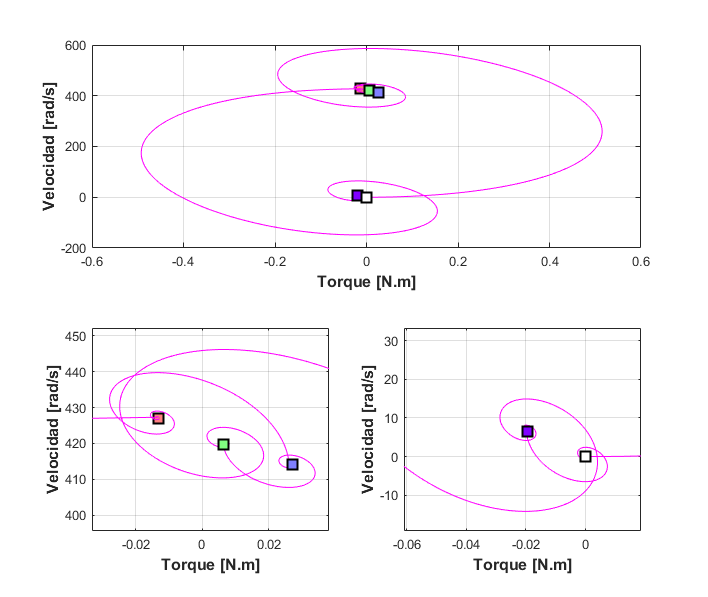
\includegraphics[width=0.7\textwidth]{T vs velocidad.png}
	\caption{\label{fig:T vs velocidad} Curva paramétrica $T_{m}$ vs $\omega_{m}$.}
	\end{figure}
	
	\item \textbf{Determinación de velocidad y corriente final de establecimiento luego de cada transitorio, especificaciones en el dominio del tiempo.}
	
	En la siguiente tabla \ref{tab:1} y \ref{tab:2} se muestra los parámetros que caracterizan las respuesta del sistema en el dominio del tiempo.
	\begin{table}[!h]
	\begin{center}
	\begin{tabular}{| c | c | c | }
	\hline
	  & Escalón $v^{r}_{qs}=19.596 V$& Escalón $T_{l}=6.28 N.m$\\ \hline
	 $\omega_{establecimiento} (rad/s)$ &  420.5 &  414.2 \\ \hline
	 Rise Time (s) &  0.0041 &  0.0015\\ \hline
	SettlingTime (s)& 0.0437 & 0.0498 \\ \hline
	Overshoot & 39.44$\%$ & 103.15$\%$ \\ \hline
	\end{tabular}
	\caption{Parámetros temporales $\omega_{m}$}
	\label{tab:1}
	\end{center}
	\end{table}
	
	\begin{table}[!h]
	\begin{center}
	\begin{tabular}{| c | c | c | }
	\hline
	  & Escalón $v^{r}_{qs}=19.596 V$& Escalón $T_{l}=6.28 N.m$\\ \hline
	 $ i^{r}_{qs}$ Establecimiento (A) &   0.09067 &  0.38 \\ \hline
	 Rise Time (ms) &  0.0026 &  4.1\\ \hline
	SettlingTime (s)& 0.048 & 0.0437 \\ \hline
	Overshoot & 8056.7$\%$ & 39.44$\%$ \\ \hline
	Sobre pico & 7.404 & 0.489 \\ \hline
	\end{tabular}
	\caption{Parámetros temporales $i^{r}_{qs}$}
	\label{tab:2}
	\end{center}
	\end{table}
	
	Como se puede apreciar ambas entradas tienen influencia sobre $ i^{r}_{qs}$ y $\omega_{m}$, sin embargo es notorío que la tensión tiene una mayor influencia sobre el valor de la velocidad al menos una vez pasados los transitorios, pero para $ i^{r}_{qs}$el torque de carga tiene una mayor influencia sobre esta. Esta relación se puede encontrar fácilmente el teorema del valor límite, en la ec .\ref{eq:2.1.2.i.2} se aplica a $\omega_{m}$, y se puede ver claramente que el valor estacionario es proporcional con la tensión y que es inversamente proporcional con el torque de carga. Además se puede concluir también que el peso de $T_{l}$ es menor, ya que el denominador se encuentra afectado por la inversa de r.
	
	\begin{equation}
	\omega_{estable}=\frac{\frac{3}{2}P_{p}\lambda^{r'}_{m}}{\frac{3}{2}P^{2}_{p}\lambda^{r'2}_{m}+ R_{s}b_{eq}}V^{r}_{qs}(0) -  \frac{R_{s} \frac{1}{r}}{\frac{3}{2}P^{2}_{p}\lambda^{r'2}_{m}+ R_{s}b_{eq}}T_{l}(0)
	\label{eq:2.1.2.i.2}
	\end{equation}
	
	%\item \textbf{Comparar comportamiento de $i^{r}_{ds}(t)$ para $i^{r}_{ds}(0)=\pm  0.5 A$ vs $i^{r}_{ds}(0)=0A$ }
	\item \textbf{Field forcing and weakening a lazo abierto }
	
	Por último, se aplica una consigna de tensión en el eje d, $v^{r \ *}_{ds}(t)=\pm 1.9596 V_{cc}$ en $t=0.5 s$ para el evaluar el efecto de reforzamiento y debilitamiento de campo. En las figuras \ref{fig:Tdistintode0} y \ref{fig:wdistintode0} se puede observa el efecto de este para el \textbf{modelo NL desacoplado con Ley de control NL} sobre el torque y la velocidad.\\
	Se puede observar claramente lo comentado en el inciso \textbf{2.1.2.d} al aplicar a tensión consigna $v^{r \ *}_{ds}(t)= 1.9596 V_{cc}$ se produce un reforzamiento del campo aumentando el torque y disminuyendo la velocidad, por otro lado si la consigna de tensión es  $v^{r \ *}_{ds}(t)= -1.9596 V_{cc}$ se produce un debilitamiento del campo disminuyendo el torque motor y aumentando la velocidad (en este caso esto se ve incrementado aún mas por el torque de carga). 
	
	
	\begin{figure}[h!]
	\centering
	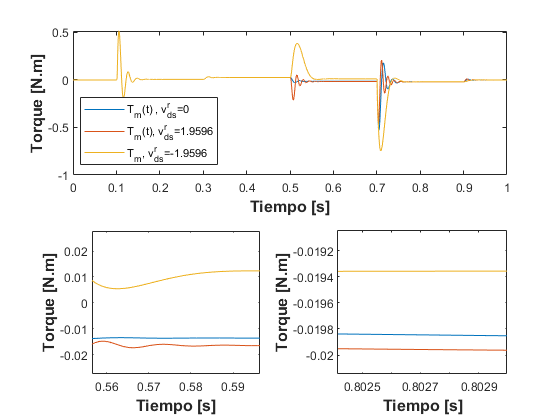
\includegraphics[width=0.7\textwidth]{Tdistintode0.png}
	\caption{\label{fig:Tdistintode0} Field forcing and weakening $T_{m}$. Modelo NL desacoplado con Ley de control NL .}
	\end{figure}
	
	\begin{figure}[h!]
	\centering
	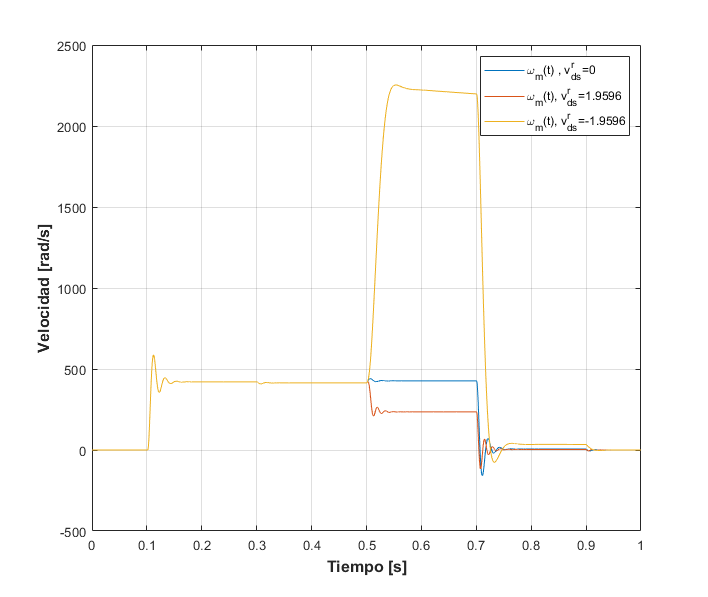
\includegraphics[width=0.7\textwidth]{wdistintode0.png}
	\caption{\label{fig:wdistintode0} Field forcing and weakening $\omega_{m}$. Modelo NL desacoplado con Ley de control NL .}
	\end{figure}
	
	Lo mismo se puede ver que ocurre para el \textbf{modelo LTI equivalente aumentado} aunque en menor medida en la figura \ref{fig:Tdistintode0LTI}, esto se debe a que en este modelo se desacopla la influencia de $i^{r}_{ds}$ sobre el eje q y por lo tanto solo influye en el torque por el siguiente término: $(L_{d}-L_{q}).i^{r}_{ds}(t).i^{r}_{qs}(t)$ y dado que por ser un motor síncrono de polos salientes $L_{d}$ y $L_{q}$ son muy parecidas la ganancia de este término es ínfima en comparación a los demás.
	
	\begin{figure}[h!]
	\centering
	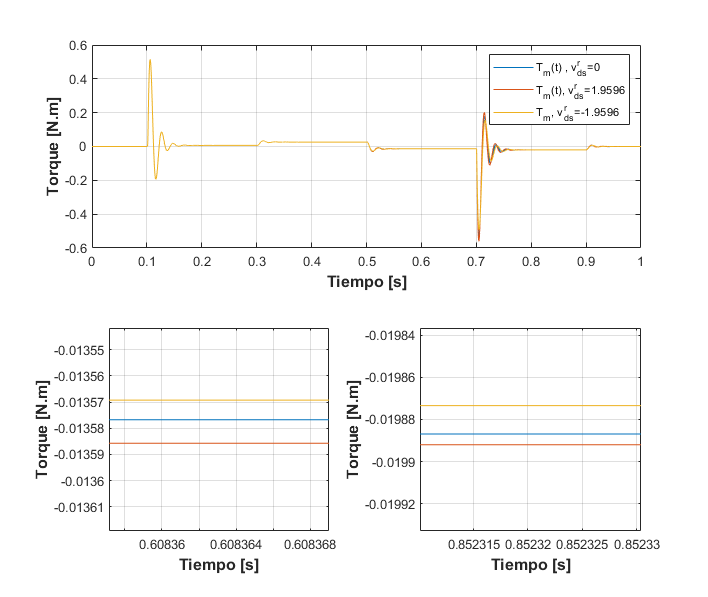
\includegraphics[width=0.7\textwidth]{Tdistintode0LTI.png}
	\caption{\label{fig:Tdistintode0LTI} Field forcing and weakening $T_{m}$. Modelo LTI equivalente aumentado.}
	\end{figure}
\end{itemize}

\subsection{Diseño, Análisis y Simulación con CONTROLADOR de Movimiento en Cascada con Modulador de Torque equivalente (Control Vectorial)}
\begin{itemize}
\item \textbf{Desacoplamiento de todas las realimentaciones físicas naturales de estado hacia la entrada}
	 En la figura \ref{fig:Tmodulado} se puede observar el desacoplamiento de todas las realimentaciones. Se ha remarcado en rojo la \textbf{La ley de control mínima} que anteriormente se implementó en el modelo NL y en naranja la \textbf{Ley de control complementaria mínima en el eje q}  que se implementó en el modelo LTI equivalente aumentado, es decir que podría decirse que los modelos realizados anteriormente son un caso particular de realizar el desacoplamiento de las realimentaciones físicas. En gris se nuestra el desacople de las caídas ohmicas, en verde la caida por tensión inducida producto de $\lambda^{`r}_{m}$ y en celeste se ha desacoplado el torque por fricción.

	\begin{figure}[h!]
	\centering
	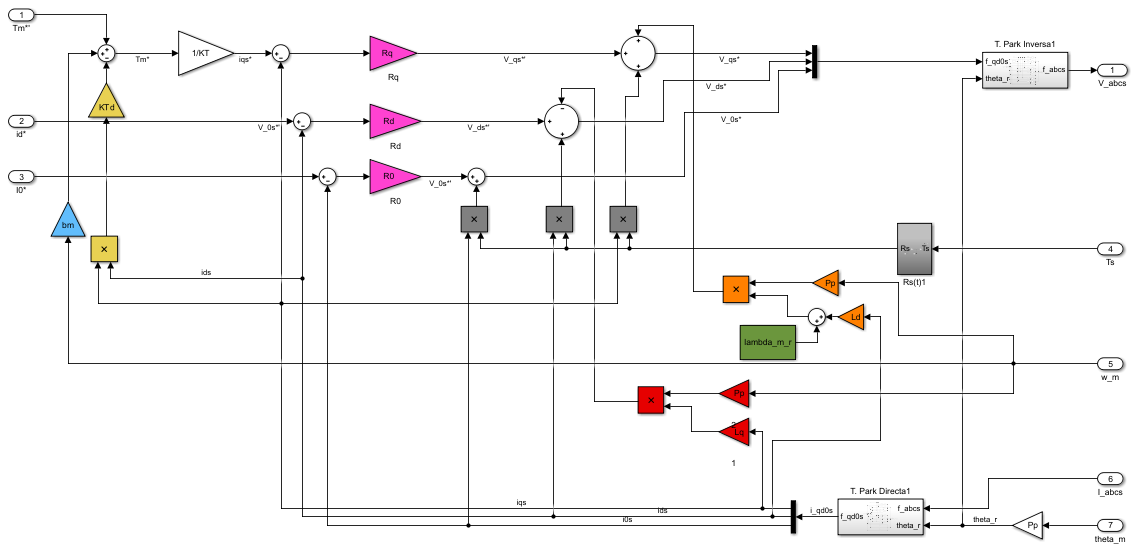
\includegraphics[width=\textwidth]{modulador de torque.png}
	\caption{\label{fig:Tmodulador}Modulador de Torque equivalente. Desacoplamiento de todas las realimentaciones físicas naturales.}
	\end{figure}
	
	En la figura \ref{fig:Ts} podemos ver el efecto de la temperatura sobre la resistencia $R_{s}$, si la temperatura tiene variaciones importantes, como vemos la resistencia no, por lo que se podría considerar constante sin caer en grandes errores. 
	
	\begin{figure}[h!]
	\centering
	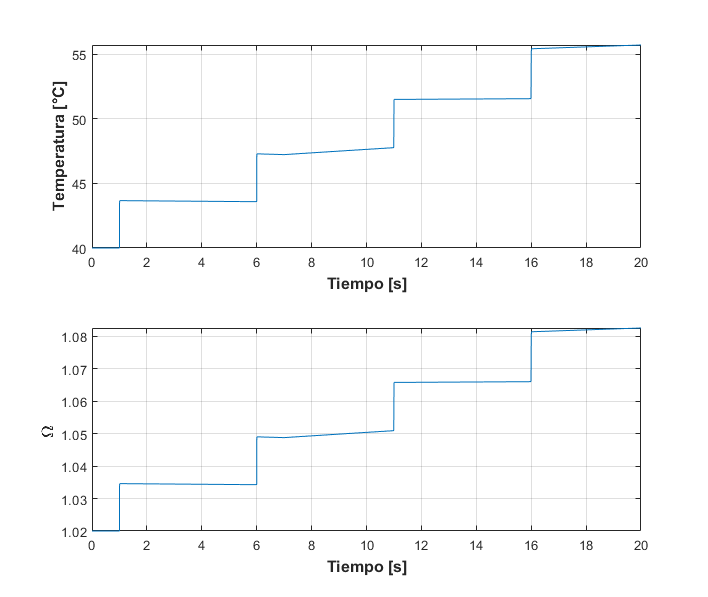
\includegraphics[width=0.7\textwidth]{Ts.png}
	\caption{\label{fig:Ts}Modulador de Torque equivalente.Desacoplamiento de todas las realimentaciones físicas naturales.}
	\end{figure}

\item \textbf{Diseño de lazos de control de corrientes $i^{r}_{qd0s}$}
Se realizará el desarrollo matemático del lazo de corriente.Considerando que el modulador de tensión es lo suficientemente rápido, exacto y su ganancia es unitaria (ec. \ref{eq:2.1.2.k.1}).
	\begin{equation}
	v^{*}_{qs}(t)\simeq v_{qs}(t)
	\label{eq:2.1.2.k.1}
	\end{equation}
y teniendo en cuenta los desacoples realizados en el punto anterior:
	\begin{equation}
	v^{*}_{qs}(t)= v^{*'}_{qs}(t) + R_{s}. i_{qs}(t) + [\lambda^{r'}_{m}+L_{d}.i^{r}_{ds}(t)].\omega_{m}(t)
	\label{eq:2.1.2.k.2}
	\end{equation}
Reemplazando la ec. \ref{eq:2.1.2.k.1} y ec. \ref{eq:2.1.2.k.2} en ec.\ref{sist:electrico1} obtenemos:
\begin{equation}
	\frac{di^{r}_{qs}(t)}{dt} . L_{q}= v^{*'}_{qs}(t)
	\label{eq:2.1.2.k.3}
	\end{equation}
	Donde la consigna $v^{*'}_{qs}(t)$ se define proporcional al error de corriente y con una ganancia proporcional. Por tanto el lazo de corriente para $i^{r}_{qs}(t)$ se define como:
	\begin{equation}
	\frac{di^{r}_{qs}(t)}{dt} . L_{q}= v^{*'}_{qs}(t)=(i^{r*}_{qs}(t)-i^{r}_{qs}(t))*Rq
	\label{eq:2.1.2.k.4}
	\end{equation}
	
	y su función de transferencia es:
		\begin{equation}
	\frac{I^{r*}_{qs}(t)}{I^{r}_{qs}(t)}=\frac{1}{s\frac{L_{q}}{R_{q}}+1}
	\label{eq:2.1.2.k.5}
	\end{equation}
	
	Podemos observar que el lazo de la ex.\ref{eq:2.1.2.k.5} presenta un polo en $s=-\frac{R_{q}}{L_{q}}$. Por ende, definiendo el parámetro $R_{q}$ podemos ubicar el polo en $s=-5000[rad/s]$, asi:\\
	$R_{q}=5000 . L_{q}=29\Omega$
	
	De las misma forma se determinan las ganancias para los otros lazos de corrientes, obteniendo:\\
	$R_{d}=5000 . L_{d}=33\Omega$\\
	$R_{0}=5000 . L_{ls}=4\Omega$\\
	
	Si comparamos con la dinámica de los modelos analizados en la \textbf{sección 2.1.6} veremos que las respuestas de las corrientes $i^{r}_{qd0s}$ son muchos mas rápidas y sin oscilaciones, ya que, esto es lo que se quiso cuando se eligió el polo para estos lazos. Asi si se tiene un $i^{r}_{ds}(0)\neq 0$ veremos que el decaimiento de esta es mucho mas rápida, también la respuesta ante una entrada consigna para $i^{r}_{qs}$ donde en la tabla \ref{tab:3} se puede observar que sus características temporales son muchos mejores que las calculadas en la tabla \ref{tab:2}
		\begin{table}[!h]
	\begin{center}
	\begin{tabular}{| c | c | c | }
	\hline
	  & Escalón $i^{r*}_{qs}$\\ \hline
	 $ i^{r}_{qs}$ Establecimiento (A) &   0.09067 \\ \hline
	 Rise Time (ms) &  0.439\\ \hline
	SettlingTime (ms)& 0.78\\ \hline
	Overshoot &0$\%$ \\ \hline
	\end{tabular}
	\caption{Parámetros temporales $i^{r}_{qs}$}
	\label{tab:3}
	\end{center}
	\end{table}
	
\item \textbf{Incorporación adecuada de consigna de torque}\\
Si idealizamos el problema y consideramos que los valores físicos modelados son iguales a los valores físicos reales y teniendo en cuenta el desacoplamiento y los lazos de corrientes calculados anteriormente, obtenemos control directo sobre las corrientes lo que nos permitirá realizar el control vectorial del campo imponiendo consignas de corriente en directo nula (o también realizar un reforzamiento o debilitamiento del campo principal) e imponer una consina de corriente en cuadratura $i^{r}_{qs}(t)$ o  lo que es lo mismo, una consigna de torque motor $T_{m}$ multiplicado por la constante de escala $1/K_{T}$ (ec.\ref{eq:2.1.2.k.6}). Hay que tener en cuenta que el lazo de corriente ($BW=1000Hz$) no es lo suficientemente rápido como se quisiera ($BW=796Hz$).
		\begin{equation}
	K_{T}=\frac{3}{2}P_{p}\lambda^{r}_{m}
	\label{eq:2.1.2.k.6}
	\end{equation}
	También hay que observar que en nuestro modulador de Torque (figura \ref{fig:Tmodulador}) se desacopla el torque generado por la fricción viscosa del motor y la caja (en celeste). Asi:
			\begin{equation}
	i^{r*}_{qs}(t)=\frac{1}{K_{t}}[T^{*'}_{m}+b_{m}\omega_{m}(t)]=T^{*}_{m}
	\label{eq:2.1.2.k.7}
	\end{equation}
	
	En la figura \ref{fig:TTmodulador_id} se dio una consigna de $T_{m}=0.0063$ y un $T_{l}$ igual al que se propuso en la sección \textbf{2.1.6}, se puede observar el aumento del torque motor al hacer el reforzamiento de campo con $i^{r}_{ds}(t)=1 A$ y en la figura \ref{fig:vqmodulador_id} se puede notar el cambio en la tensión en el eje q producto de esta corriente. Se puede concluir que este reforzamiento no produce mejoras significativas sobre el torque motor a comparación con el considerable aumento que se genera en la tensión del eje q.
	 	\begin{figure}[h!]
	\centering
	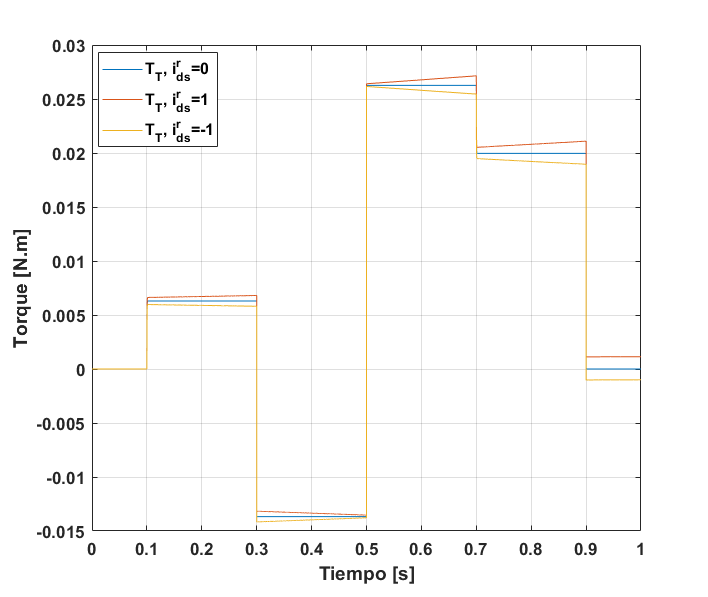
\includegraphics[width=0.7\textwidth]{TTmodulador_id.png}
	\caption{\label{fig:TTmodulador_id}Torque motor para $i^{r}_{ds}\neq0$.}
	\end{figure}
		 	\begin{figure}[h!]
	\centering
	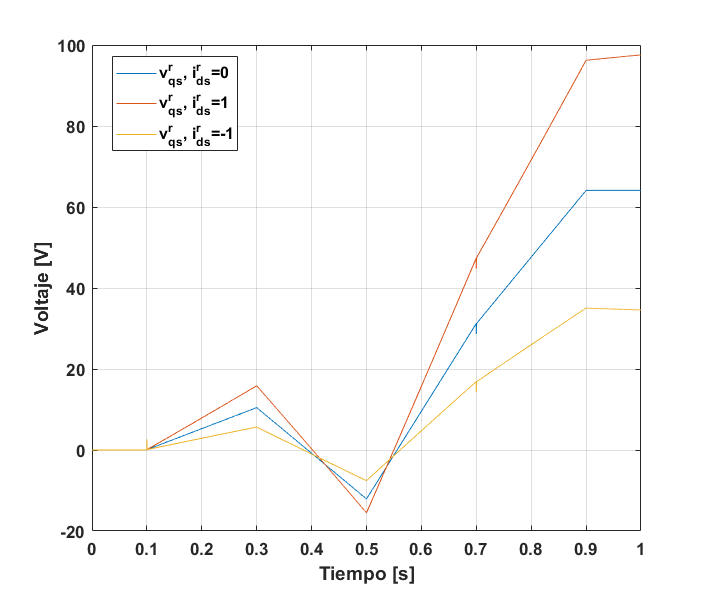
\includegraphics[width=0.7\textwidth]{Tmodulador_id.png}
	\caption{\label{fig:vqmodulador_id}$v^{r}_{qs}$ requerida para una $i^{r}_{ds}\neq0$.}
	\end{figure}
\end{itemize}
\subsubsection{Controlador externo de movimientos: posición/velocidad }
Acontinuación se diseñará el controlador utilizando el método de sintonía serie con acción integral (``PID''), con $n=2.5$ y $\omega_{pos}=800\frac{rad}{s}$. Para obtener la ecuaciación de transferencia del sistema con el controlador de movimiento partiremos del modulador de torque obtenido en el inciso anterior, lo que nos permite tener un acceso directo a manipular el torque motor. Considerando esto la ecuación del sistema es:
		\begin{equation}
	J_{eq}\theta(s)s^{2}+b_{leq}\theta(s)s=T^{`}_{m}(s)-T_{leq}(s) \ ; \ b_{leq}= \frac{b_{l}}{r^{2}} \ ; \ T_{leq}= \frac{T_{l}}{r}
	\label{eq:2.1.2.q.1}
	\end{equation}
La ecuación del controlador PID es:
		\begin{equation}
	T^{*`}_{m}(s)=e_{w}(s)[ba+\frac{1}{s}Ksa + \frac{1}{s^{2}}Ksia]
	\label{eq:2.1.2.q.2}
	\end{equation}
Recordando la ec.\ref{eq:2.1.2.k.7} y la ec. \ref{eq:2.1.2.k.5} se obtiene:

	\begin{equation}
	T^{`}_{m}(s)=\frac{1}{\frac{L_{q}}{R_{q}}s+1}T^{*'}_{m}(s) \ ; \ G_{I}(s)=\frac{L_{q}}{R_{q}}s+1
	\label{eq:2.1.2.q.4}
	\end{equation}

	\begin{equation}
	J_{eq}\theta(s)s^{2}+\frac{b_{l}}{r^{2}}\theta(s)s=G_{I}(s)e_{w}(s)[ba+\frac{1}{s}Ksa + \frac{1}{s^{2}}Ksia]-T_{leq}(s)
	\label{eq:2.1.2.q.5}
	\end{equation}
	
Asi obtenemos:
 
	\begin{equation}
	G_{\theta^{*}_{m}}(s)=\frac{G_{I}(s)[s^{2}ba+sKsa+Ksia]}{J_{eq}s^{3}+b_{leq}s^{2}+G_{I}(s)[s^{2}ba+sKsa+Ksia]}
	\label{eq:2.1.2.q.6}
	\end{equation}
 	\begin{equation}
	G_{T_{leq}}(s)=\frac{s}{J_{eq}s^{3}+b_{leq}s^{2}+G_{I}(s)[s^{2}ba+sKsa+Ksia]}
	\label{eq:2.1.2.q.6}
	\end{equation}
	
	Si consideramos que el lazo de corriente es lo suficientemente rápido $G_{I}\equiv 1$, entonces los polos del sistema se determinan por el polinomio característico:
	\begin{equation}
	P_{c}=J_{eq}s^{3}+[b_{leq}+ba]s^{2}+sKsa+Ksia
	\label{eq:2.1.2.q.7}
	\end{equation}
	
	Haciendo uso del método de sintonía serie:\\
	$ n\omega_{pos}=\frac{ba+b_{leq}}{J_{eq}} \ ; \ ba=n\omega_{pos}J_{eq}-b_{leq}$ \\
	$ n\omega^{2}_{pos}=\frac{Ksa}{J_{eq}} \ ; \  Ksa=n\omega^{2}_{pos}J_{eq} $\\
	$ \omega^{3}_{pos}=\frac{Ksia}{J_{eq}} \ ; \  Ksia=\omega^{3}_{pos}J_{eq} $\\
	
	Si consideramos los valores nominales de $J_{l}$ y $b_{l}$ se tiene:\\
	$ba=0.0113 \frac{N.m}{\frac{rad}{s}}$\\
	$Ksa=9.04 \frac{N.m}{rad}$\\
	$Ksia=2892.8 \frac{N.m}{rad.s}$\\
	
	Se busca asi tener un controlador PID que no haga uso de bloques derivativos, para no tener una amplificación de ruido. Por esto, en el caso de definir un perfil de posición $q^{*}(t)$, será necesario derivar el perfil.
	En la figura \ref{fig:controladorPID} se observa el diagrama en bloques del controlador PID.
		 	\begin{figure}[h!]
	\centering
	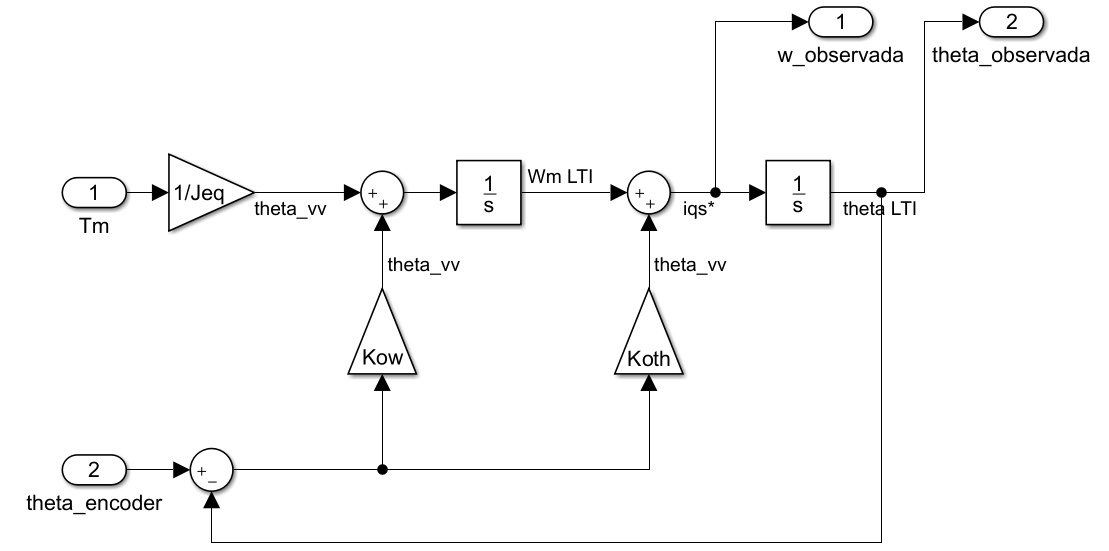
\includegraphics[width=0.7\textwidth]{controladorPID.png}
	\caption{\label{fig:controladorPID}Controlador PID.}
	\end{figure}
	
	La gráfica de los polos del controlador el regulador de corriente y los polos de la planta original se muestran en la figura\ref{fig:Polosmodelos}, adonde se puede ver que el lazo de corriente es mucho mas rápido que los demás y que los polos del controlador son más rápidos que los de la planta original.
			 	\begin{figure}[h!]
	\centering
	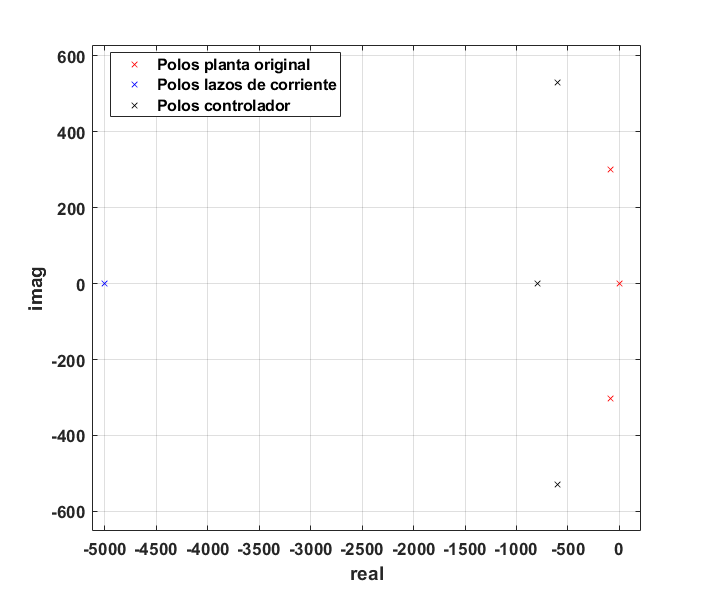
\includegraphics[width=0.7\textwidth]{Polosmodelos.png}
	\caption{\label{fig:Polosmodelos}Polos de la planta, lazo de corriente y controlador PID.}
	\end{figure}
	
	Dados que los polos en la figura \ref{fig:Polosmodelos} fueron graficados para valores nominales de $J_{l}$ y $B_{l}$ y que estos valores nominales pueden variar dentro de los límites especificados por la aplicación, se realizó un análisis de la migración de los polos del controlador con la variación de estos parámetros. La variación de $B_{l}$ no tuvo prácticamente reprecusión sobre los polos del sistema. Pero la variación de $J_{l}$, si produjo cambios considerables sobre los polos de este (figura \ref{fig:PoloJeq}), es por esto que se puede concluir, que el controlador, si bien es estable para todo valor considerado de los parámetros, la inercia presenta una gran influencia sobre la estabilidad de este, por lo que no se descarta que en caso de poseer mayores variaciones sea necesario recurrir a estrategias de control que se adapten en función de la inercia variable del sistema.
	\begin{figure}[h!]
	\centering
	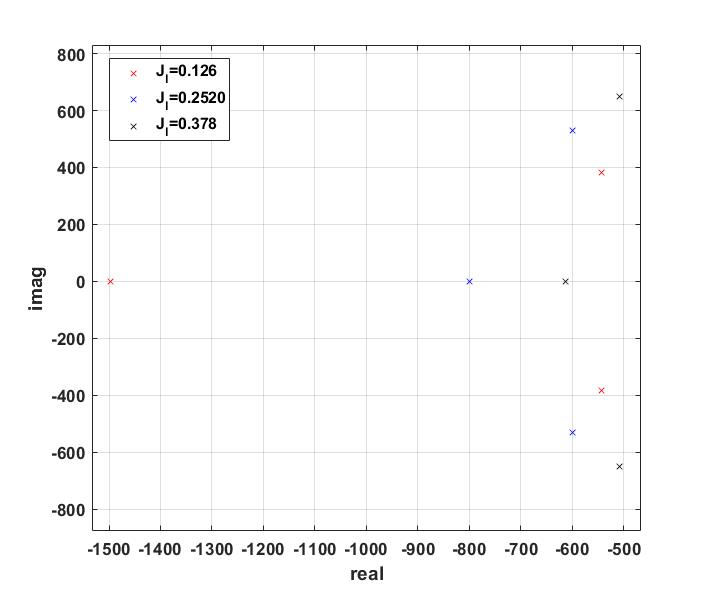
\includegraphics[width=0.7\textwidth]{PoloJeq.png}
	\caption{\label{fig:PoloJeq}Variación de los polos del controlador con $J_{l}$.}
	\end{figure}
	

\subsubsection{Incorporación y diseño de Observador de Estado de orden reducido sólo para la parte mecánica de este controlador}
Trubii
\subsubsection{Simulación en tiempo continuo con modelo completo NL}
\begin{itemize}
	\item \textbf{Seguimiento de consignas}

Para la simulación del sistema se utilizará un perfil trapezoidal 
de posición 
$\omega_{l}=q1*(t) \equiv \frac{1}{r}\theta^{*}_{m}(t)$ con $q_{1}^{*}(t)=0 \rightarrow (\Delta t_{ramp}=5s) \rightarrow 2.\pi [rad] \rightarrow (\Delta t_{ramp}=5s) \rightarrow 0$. Como vemos se plantea un giro completo de la articualción en 5s
del robot con una velocidad constante y luego la vuelta de la misma a la posición cero.
En la figura \ref{fig:consigna} se puede observar el seguimiento de la consigna dada y en la figura \ref{fig:consigna2} se muestra la velocidad angular. Como vemos las consigna se siguen correctamente.
Pero se puede observar que hay sobrepicos en ambas figuras, esto se debe a que la señal de consigna elegida no es la mejor, ya que como se ve, en los quiebres bruscos de posición
se producen escalones de velocidad, lo que a su vez generan impulsos muy grandes de aceleración y esto es lo que produce el gran overshot visto sobre todo en la velocidad.

\begin{figure}[h!]
	\centering
	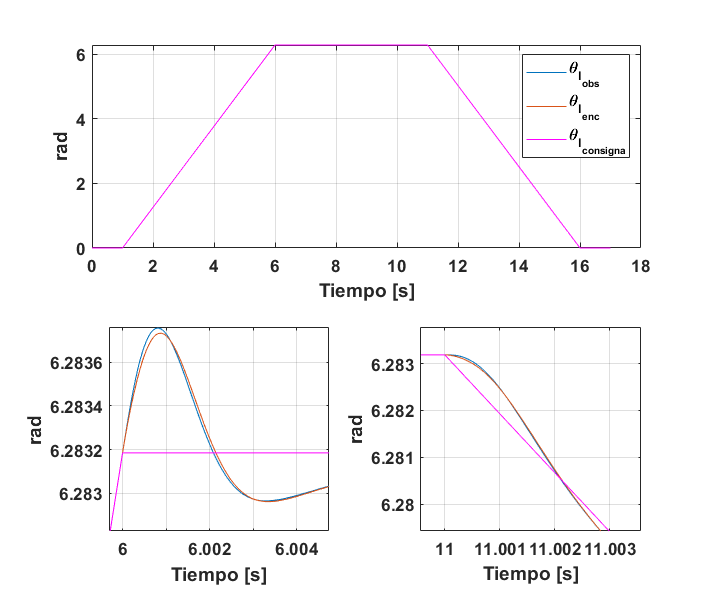
\includegraphics[width=0.7\textwidth]{consigna.png}
	\caption{\label{fig:consigna}Posición angular sensada, observada y consigna.}
	\end{figure}

\begin{figure}[h!]
		\centering
		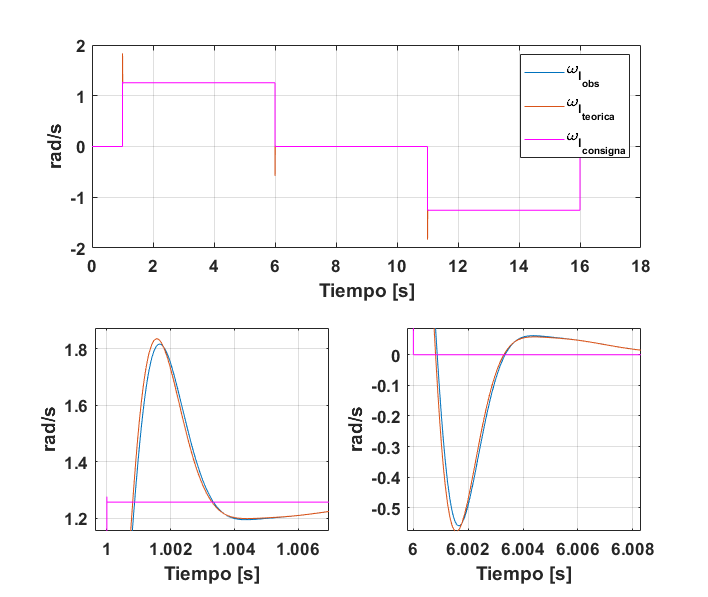
\includegraphics[width=0.7\textwidth]{consigna2.png}
		\caption{\label{fig:consigna2}Velocidad angular teórica, observada y consigna.}
		\end{figure}


	\item \textbf{Rechazo a perturbaciones}
	
	Se analizará la respuesta del sistema ante cargas externas, considerando valores nominales y variación máxima de los parámetros de carga mecánica física.
	Para observar mas facilmente los efectos de las perturbaciones se da una consigna de torque motor nula y se perturba al sistema con $T_{l}=6.28 N.m$.
	
	En la figura \ref{fig:perturbaciones} se puede ver que el sistema presenta un error estacionario ante una perturbación y también que este varía al cambiar los parámetros de carga, en este caso $J_{l}$, vemos además que la mayor variación se da en el transitorio. Por otro lado al variar $b_{l}$ no se notaron cambios por lo que no se grafico. Sin embargo, se puede apreciar que el rechazo a las perturbaciones es prácticamente igual 
	por lo que el sistema es robusto ante el cambio de estos parámetros dentro de los límites considerados.
	Y el error se da a causa de implementar un observador PD, el mismo no es capaz de rechazar las perturbaciones del sistema.
	\begin{figure}[h!]
		\centering
		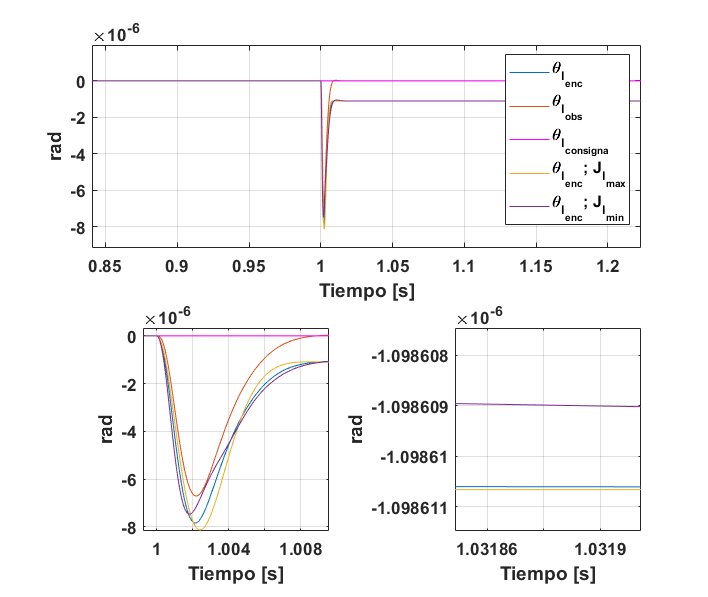
\includegraphics[width=0.7\textwidth]{perturbaciones.png}
		\caption{\label{fig:perturbaciones}Posición angular sensada, observada y consigna.}
		\end{figure}
	\end{itemize}
\subsubsection{Verificación de desempeño y/o mejoras}
\begin{itemize}
	\item \textbf{Verificar si se supera/n alguna/s de las Especificaciones de operación}
	En la siguiente tabla se visualizará los valores alcansados por las variables del sistema y sus límites.
	\begin{table}[!h]
		\begin{center}
		\begin{tabular}{| c | c | c | }
		\hline
		  & Valores medidos & Valor nominal  \\ \hline
		 Tension de fase (V) & 1889 (Pico), 18.4 (R. continuo) & 13.86\\ \hline
		 Vel. rotor [rad/s]& 577 (Pico) 395 (R. continuo)&  691.15\\ \hline
		Corriente R. continuo (A) &0.089 & 0.4\\ \hline
		Corriente corta duración (A) &49.33 &2\\ \hline
		Temperatura (°C) &54.1 & 115\\ \hline
		Torque corta duración (N.m) & 1425 & 29.42\\ \hline
		Torque R. continuo (N.m) & 0.0757 & 7.26\\ \hline
		\end{tabular}
		\caption{Variables del sistema}
		\label{tab:4}
		\end{center}
		\end{table}
En la figura \ref{fig:parametros} se muestra distinta variables internas de la planta.
\begin{figure}[h!]
	\centering
	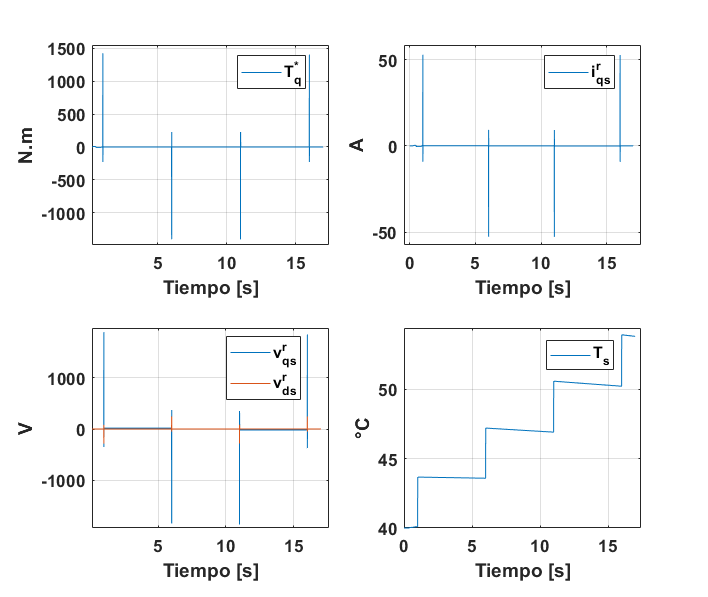
\includegraphics[width=0.7\textwidth]{parametros.png}
	\caption{\label{fig:parametros}Torque, corriente, tensión y temperatura.}
	\end{figure}

Como se muestra en la tabla \ref{tab:4} el sistema, para la consigna planteada, supera ampliamente los límites establecidos,
 por lo que es necesario remendar esta situación ya que si se opera en esta condiciones, se dañaría gravemente al sistema.
 Se puede concluir que la causa de esto es la consigna de posición sugerida, ya que, esta sobre exige al sistema provocando que este opere fuera 
 de sus límites.

 De esta manera se procedió a cambiar la forma de esta consigna, elegiendo un perfil trapezoidal de velocidad para el cual vamos a tener en cuenta las siguientes restricciones:
 \begin{itemize}
	 \item Restricción de velocidad: Como ya se mencionó anteriormente la velocidad es directamente proporcional a la tensión por lo que en el caso de neustro motor la velocidad 
	 va a estar limitada por la tensión máxima de fase admisible, la cual es \textbf{$V_{sfnom}=13.86 V$}, la cual a partir de la ec.\ref{eq:2.1.2.i.2} nos permite calcular nuestra velocidad
	 máxima, la cual es $\omega_{m}=298.76\frac{rad}{s}$, de esta manera esta queda limitada por el subsistema electrico y no por la parte mecánica, ya que, el tren de transmisión nos 
	 permite una $\omega_{m}=691.15\frac{rad}{s}$.

	 \item Restricción de aceleración: El torque motor es proporcional a la corriente y a su vez es proporcional a la aceleración, por ende la aceleración del perfil consigna elegiendo
	 va a estar limitada por las corrientes nominales y picos establecidas por el fabricante.

	 \item Restricción de Jerk: Si bien en las especificaciones de nuestra aplicación no se limita este, es un parámetro muy importante a tener en cuenta ya que es lo que determina las sacudidas 
	 que se producen sobre el sistema y es la resistencia mecánica de la articulación la que determina su valor máximo permitido. Además con se podrá apreciar un perfil trapezoidal de velocidad
	 produce sobrepicos en la aceleración, por lo que si se quiere minimizar este efecto, este perfil no es el mejor.

 \end{itemize}

 Teniendo en cuenta las restricciones anteriormente planteadas, y que la velocidad mínima para realizar la consigna demandada es $\omega_{m}=395[\frac{rad}{s}]$, concluimos que esta consigna no es alcanzable
 por nuestro sistema, por lo que aumentamos $\Delta t_{ramp}$ a 6s, para el cual necesitaríamos un $\omega_{m}=332[\frac{rad}{s}]$ lo cual sigue estan fuera de nuestros límites, por ende se propone hacer un debilitamiento
 de campo con $i^{r}_{ds}=-0.4A$ lo que provoca que nuestro límite de velocidad pase a ser $\omega_{m_{max}}=355$, por lo tanto para nuestoro perfil de velocidad lo vamos a restringir para una velocidad $\omega_{m}=355[\frac{rad}{s}]\rightarrow \omega_{l}=1.13[\frac{rad}{s}]$ y 
 $\Delta t_{ramp}=6$ por lo que nuestro perfil queda como se ve en la figura\ref{fig:consignasnuevas}.
 
 \begin{figure}[h!]
	\centering
	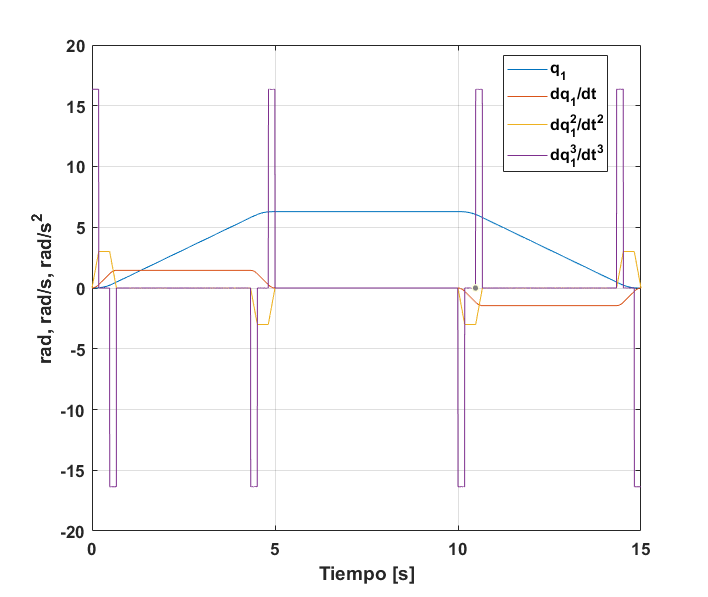
\includegraphics[width=0.7\textwidth]{consignasnuevas.png}
	\caption{\label{fig:consignasnuevas}Perfil de posición, velocidad y aceleración}
	\end{figure}

	En la figura \ref{fig:consignanuevapara} se muestran las variables del sistema ante la nueva consigna establecida.

	\begin{figure}[h!]
		\centering
		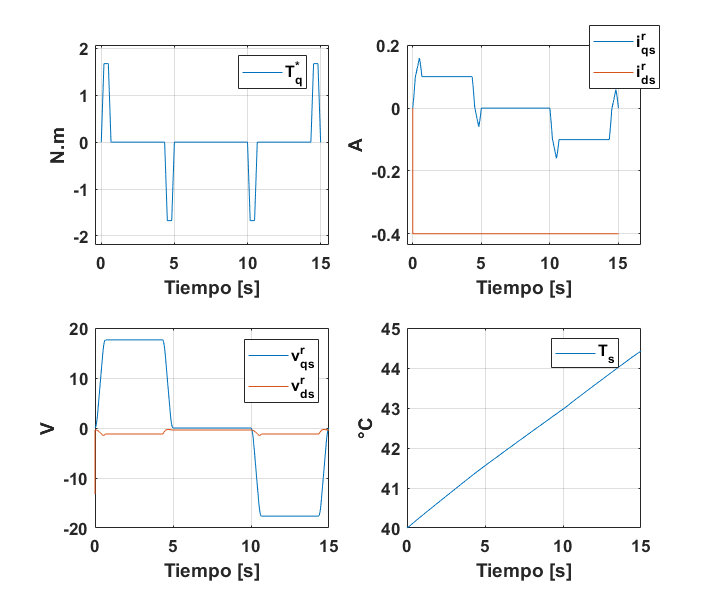
\includegraphics[width=0.7\textwidth]{consignanuevapara.png}
		\caption{\label{fig:consignanuevapara}Torque motor, corrientes de fase, temperatura y tensiones de fase}
		\end{figure}

	Las consignas de velocidad y posición son seguidas a la perfección por el motor, aunque en la velocidad se puede observar un pequeño overshot menor al 0.01 \%, y como se puede observa todas las variables estan dentro de los limites establecidos. Es bueno notar,
	 que si bien el torque y la corriente estan dentro de los límites de operación presentan overshoots notorios, por lo que ante si se qusiera disminuir las sacudidas del motor lo más posible, habría que buscar otro perfil.
	 
	Una desventaja importante del debilitamiento de campo es que se tiene una corriente $i^{r}_{ds}$ distanta de cero constane lo que provoca que la temperatura del motor suba mas rápidamente a comparación con cuando esta es nula que la temperatura prácitcamente no varía.
	
	\item \textbf{Observador agregado}
	Como ya se analizó anteriormente el observador presenta error de estado estacionario ante perturbaciones de carga dado que es un observador PD. 
	Estos no son capaces de observar las perturbaciones externas de la planta observable. Si se analiza la dinámica del error de observación:

	\begin{equation}
		\dot{e}(t)=[A-K_{e}C]e(t)+B_{d}d(t); e(t_{0})=x_{0}
		e(t)=x(t)-\tilde{x}(t)
		\label{eq:2.1.2.x.1}
	\end{equation}
	Si los polos del observador se encuentran lo suficientemente lejos del origen para hacer al observador estable y rápido, $e(t)$ tendera a ser nulo si el termino $d(t)$ es nulo, es decir si no existen perturbaciones. Este error permanete se debe a la falta de la acción integral, por tanto acontinuación se determinaran
	los nuevos polos del observador con polos ubicados en $p_{1,2,3}=-3200 \frac{rad}{s}$. 
	Siendo las nuevas ecuaciones del observador las siguientes:
	\begin{equation}
		\left\{\begin{matrix}
			\frac{d\tilde{\theta}_{m}(t)}{dt}=\tilde{\omega}_{m}(t)+K_{\theta}(\theta_{m}(t)-\tilde{\theta}_{m}(t))\\
			\frac{d\tilde{\omega}_{m}(t)}{dt}=\frac{T^{'}_{m}(t)}{J_{eq}}+K_{\omega}(\theta_{m}(t)-\tilde{\theta}_{m}(t))++K_{\omega I}\int (\theta_{m}(t)-\tilde{\theta}_{m}(t))dt
			
			\end{matrix}\right.
			\label{eq:2.1.2.x.2}
	\end{equation}
	Aplicando la transformada de Laplace a la ecuación anterior se obtiene la funciones de transeferencia de la salida $\tilde{\theta}_{m}$ respecto a las entradas $\theta_{m}$ y $\frac{T'_{m}}{J_{eq}}$. A partir de esta obtenemos el polinomio característico (ec.\ref{eq:2.1.2.x.3}) con el cual podemos definir las constantes de este para el polo deseado.

		\begin{equation}
		P_{obs}=s^{3}+K_{\theta}s^{2}+K_{\omega}s+K_{\omega I}
			\label{eq:2.1.2.x.3}
	\end{equation}

	Asi mediante la ec.\ref{eq:2.1.2.x.3} y el polinomio deseado obtenemos:\\
	$K_{\theta}=9600 \frac{1}{s}$\\
	$K_{\omega}=307.2x10^{5} \frac{1}{s^{2}}$\\
	$K_{\omega I}=3.2768 x 10^{10} \frac{1}{s^{3}}$\\

	De esta manera el diagrama de bloques del observador es el mostrado en la figura \ref{fig:observadornuevo}.
	\begin{figure}[h!]
		\centering
		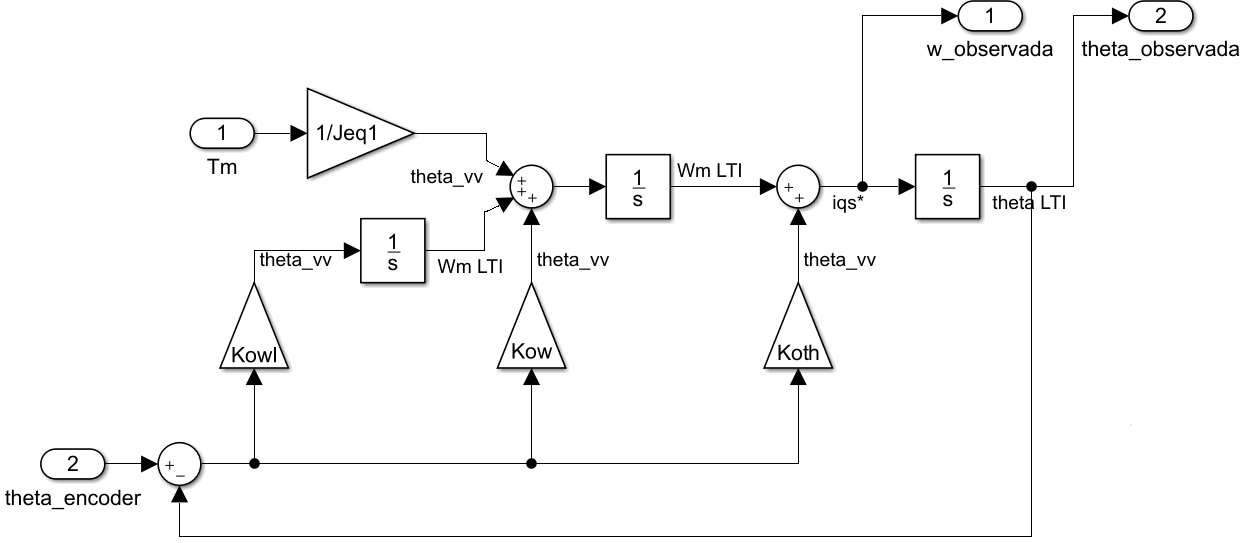
\includegraphics[width=0.7\textwidth]{observadornuevo.png}
		\caption{\label{fig:observadornuevo}Observador con acción integral}
		\end{figure}
	En la figura \ref{fig:obs} se puede observa el rechazo a una perturbación de carga para una consigna de posición igual a cero.
	\begin{figure}[h!]
		\centering
		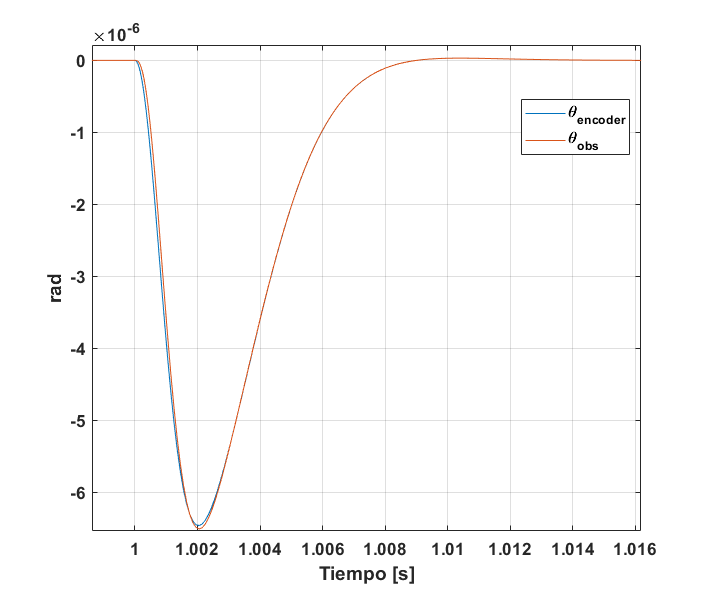
\includegraphics[width=0.7\textwidth]{obs.png}
		\caption{\label{fig:obs}Rechazo a perturbaciones de carga.}
		\end{figure}

\item \textbf{Comportamiento térmico}
Se verificó la temperatura del bobinado para una operación continua repetitiva del ciclo especificado anteriormente (figura \ref{fig:rep}) y se observó que
la temperatura se encuentra dentro de los límites de operación ha aumentado considerablemente y que si se realizan más ciclo se va a tener problemas con esta, por lo que
se concluye que si la aplicación requiere una operación del motor como la mostrada en la figura \ref{fig:rep}, no se podrá realizar el debilitamiento de campo
 opteniendo una degradación en el seguimiento de la consigna requerida, ya que el motor va a tener que operar a velocidades menores para sobrepasar los límites de tensión y es probable que 
 $\Delta t=7 s$. Por último en la figura \ref{fig:temp} se muestra la temperatura para la misma operación con y sin debilitamiento de campo, y se puede observar que el crecimiento de la temperatura
 sin debilitamiento de campo es ínfimo. Hay que aclarar que el motor no podría llevar a cabo esta consigna de movimiento sin debilitamiento de campo, ya que, se supera el límite de tensión,
  esto se ha realizado únicamente para poder comparar los distintos comportamiento.
  \begin{figure}[h!]
	\centering
	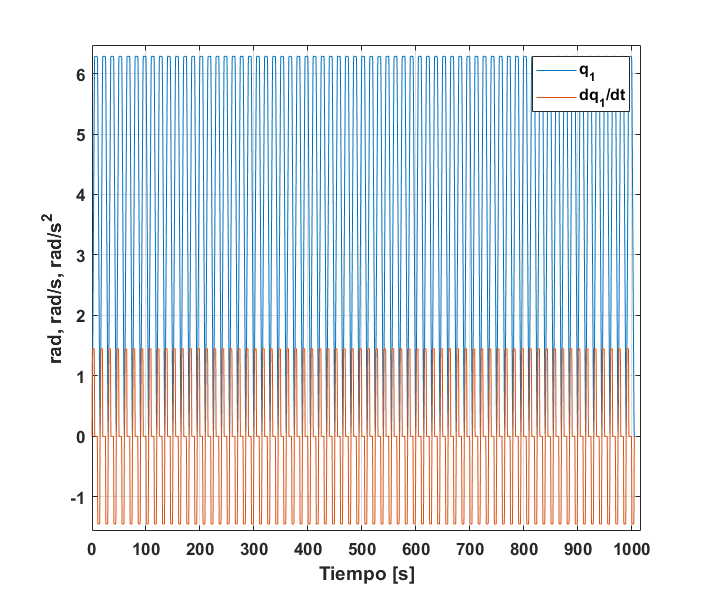
\includegraphics[width=0.7\textwidth]{rep.png}
	\caption{\label{fig:rep}Consigna de movimiento repetitiva}
	\end{figure}
	\begin{figure}[h!]
		\centering
		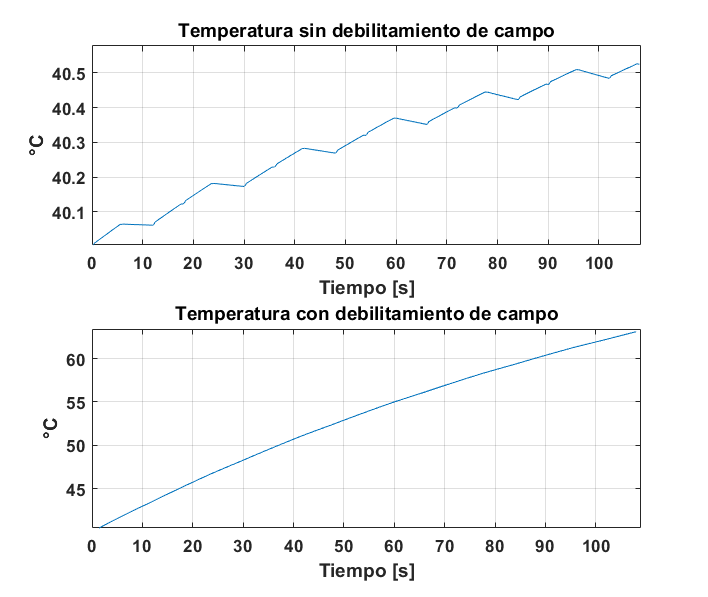
\includegraphics[width=0.7\textwidth]{temp.png}
		\caption{\label{fig:temp}Temperatura del sistema}
		\end{figure}

\item \textbf{Respuesta no ideal (ancho de banda limitado) de los sensores y acondicionadores de señal}
Se reemplaza el modelo ideal $G(s)\equiv 1$ para los sensores ausmido hasta aquí,por modelos aproximados equivalentes con características de filtro Pasa Bajos.
Para medir las corrientes de fase $i_{abcs}(t)$ y la posición angular $\theta_{m}(t)$ se plantea un modelo LP en SS de segundo orden con $\xi=1$. Para sensar la temperatura $T°_{s}(t)$ se propone un modelo LP en SS de primer orden con $\tau=20s$.

En las figuras \ref{} y \ref{} se puede ver la degradación de desempeño del sistema cuando se consideran los sensores no ideal, se puede observar que a medida que se disminuye el ancho de banda de estos
 la respuesta del sistema puede llegar hasta diverger con respecto a la deseada. Por ende se puede concluir que es algo que hay que tener muy presente en el diseño de sistemas de control, por que como se 
 aprecia en las imagen aparecen errores en los transitorios y estacionarios.
 \begin{figure}[h!]
	\centering
	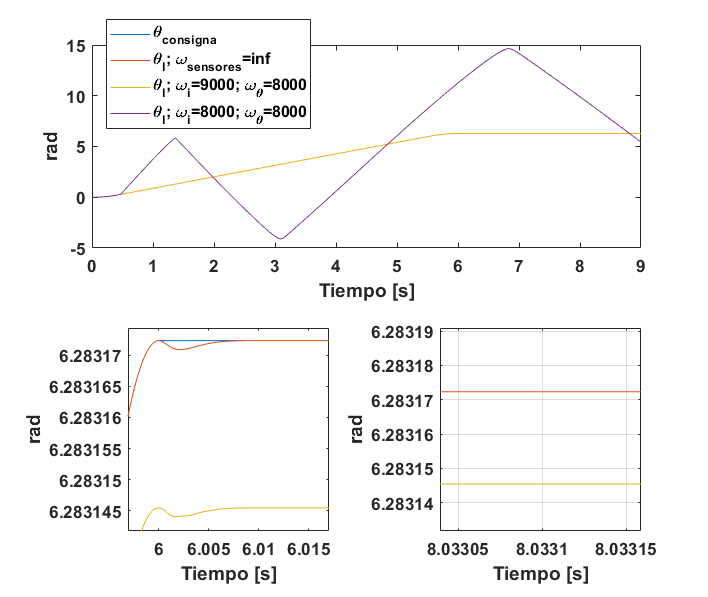
\includegraphics[width=0.7\textwidth]{theta_consignas.png}
	\caption{\label{fig:theta_consignas}Posición del sistema con sensores no ideales}
	\end{figure}
 \begin{figure}[h!]
	\centering
	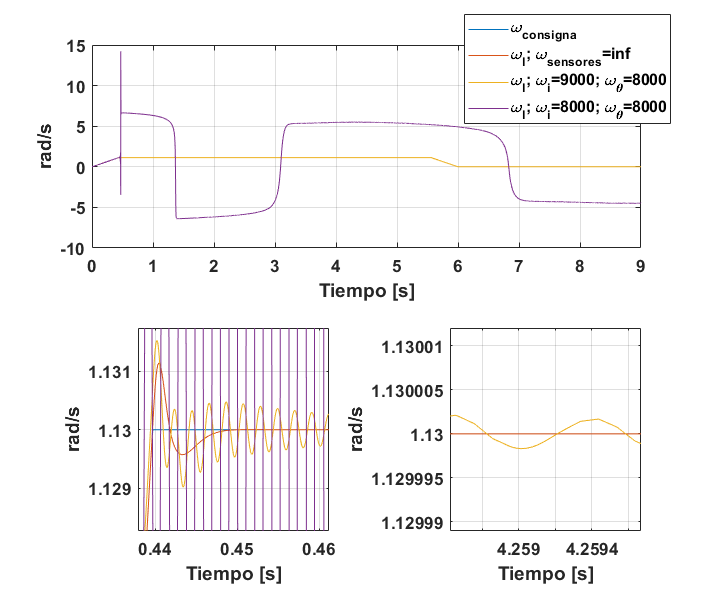
\includegraphics[width=0.7\textwidth]{omega_sensores.png}
	\caption{\label{fig:omega_sensores}Velocidad del sistema con sensores no ideales}
	\end{figure}

\end{itemize}
\section{Conclusiones}

\section{Referencias}

\end{document}